\noindent Die Fourier-Transformation erlaubt es, zeitkontinuierlichen Signalen ein Spektrum und zeitkontinuierlichen Systemen einen Frequenzgang zuzuordnen. Die Fourier-Transformation von Signalfolgen ist f\"{u}r zeitdiskrete Anwendungen das \"{A}quivalent zur bereits diskutierten Fourier-Transformation f\"{u}r zeitkontinuierliche Signale. Sie wird in diesem Kapitel eingef\"{u}hrt und ist wesentliche Voraussetzung f\"{u}r die Beschreibung zeitdiskreter Signale sowie die Analyse zeitdiskreter Systeme im Frequenzbereich.\newline

\noindent Die Fourier-Transformierte von Signalfolgen kann \"{u}ber ihre Definitionsgleichung bestimmt werden. Wie bei der z-Transformation kann die eher aufwendige Bestimmung von Korrespondenzen \"{u}ber die Definitionsgleichung vermieden werden, wenn die vorliegende Signalfolge mit Rechenregeln auf Folgen mit bekannten Korrespondenzen zur\"{u}ckgef\"{u}hrt wird. Deshalb werden f\"{u}r die Fourier-Transformation von Signalfolgen die gebr\"{a}uchlichen Rechenregeln hergeleitet und der Nutzen an Beispielen aufgezeigt. Weiterhin weist die Fourier-Transformation von Signalfolgen Symmetrien auf, die berechnet und an einem Beispiel verdeutlicht werden.\newline

\noindent Abschlie{\ss}end wird ein Zusammenhang zwischen der Fourier-Transformation von Signalfolgen, der zeitkontinuierlichen Fourier-Transformation und der z-Transformation hergestellt. 

\subsection{Grundlagen}

\subsubsection{Eigenfunktionen zeitdiskreter LTI-Systeme}

\noindent Lineare Differenzengleichungen mit konstanten Koeffizienten beschreiben zeitdiskrete LTI-Systeme. Die L\"{o}sungen dieser Differenzengleichungen setzen sich aus Exponentialfolgen zusammen. Eine besondere Stellung nehmen komplexe Exponentialfolgen der Form 

\begin{equation}\label{eq:sevenone}
x\left[k\right]=e^{j\cdot \Omega _{0} \cdot k}
\end{equation}

\noindent ein. Sie werden als Eigenfolgen des Systems bezeichnet. Bei einer Anregung mit diesen Folgen reagiert das System mit einer Folge gleicher normierter Frequenz $\Omega_{0}$ im Allgemeinen aber unterschiedlicher Amplitude und Phase.\bigskip

\noindent
\colorbox{lightgray}{%
\arrayrulecolor{white}%
\renewcommand\arraystretch{0.6}%
\begin{tabular}{ wl{16.5cm} }
{\fontfamily{phv}\selectfont{Beispiel: Anregung eines Systems 1. Ordnung mit einer komplexen Exponentialfolge}}
\end{tabular}%
}\medskip

\noindent Ein System mit der \"{U}bertragungsfunktion

\begin{equation}\label{eq:seventwo}
G\left(z\right)=\frac{z}{z-\lambda }
\end{equation}

\noindent wird mit einem Signal 

\begin{equation}\label{eq:seventhree}
x\left[k\right]=e^{j\cdot \Omega _{0} \cdot k} \cdot \sigma \left[k\right]
\end{equation}

\noindent angeregt. Das Eingangssignal hat die z-Transformierte 

\begin{equation}\label{eq:sevenfour}
X\left(z\right)=\frac{z}{z-e^{j\cdot \Omega _{0}}}
\end{equation}

\noindent Die z-Transformierte des Ausgangssignals lautet nach den Darstellungen zur z-Transformation 

\begin{equation}\label{eq:sevenfive}
Y\left(z\right)=G\left(z\right)\cdot X\left(z\right)=\frac{z}{z-\lambda } \cdot \frac{z}{z-e^{j\cdot \Omega _{0}}}
\end{equation}

\noindent \"{U}ber Partialbruchzerlegung und R\"{u}cktransformation ergibt sich die Ausgangsfolge y[k] mit

\begin{equation}\label{eq:sevensix}
\begin{split}
y\left[k\right] &=\frac{\lambda ^{k+1} }{\lambda -e^{j\cdot \Omega _{0} } } \cdot \sigma \left[k\right]+\frac{e^{j\cdot \Omega _{0} } }{e^{j\cdot \Omega _{0} } -\lambda } \cdot e^{j\cdot \Omega _{0} \cdot k} \cdot \sigma \left[k\right]=\frac{\lambda ^{k+1} }{\lambda -e^{j\cdot \Omega _{0} } } \cdot \sigma \left[k\right]+\left. G\left(z\right)\right|_{z=e^{j\cdot \Omega _{0} } } \cdot e^{j\cdot \Omega _{0} \cdot k} \cdot \sigma \left[k\right] \\ 
&=\frac{\lambda ^{k+1} }{\lambda -e^{j\cdot \Omega _{0} } } \cdot \sigma \left[k\right]+A\left(\Omega _{0} \right)\cdot e^{j\cdot \varphi \left(\Omega _{0} \right)} \cdot e^{j\cdot \Omega _{0} \cdot k} \cdot \sigma \left[k\right]
\end{split}
\end{equation}

\noindent Das System reagiert auf die harmonischen Anregung mit der Kreisfrequenz $\Omega_{0}$ abgesehen von Einschwingvorg\"{a}ngen mit einem harmonischen Signal derselben Kreisfrequenz. F\"{u}r den Fall einer harmonischen Anregung m\"{u}ssen demnach nur das Verh\"{a}ltnis der Ein- und Ausgangsamplitude sowie die Phasenverschiebung bestimmt werden. Beide Gr\"{o}{\ss}en sind von der normierten Kreisfrequenz $\Omega_{0}$ abh\"{a}ngig. Wie bei zeitkontinuierlichen Signalen wird das Verh\"{a}ltnis der Amplituden als Amplitudengang A($\Omega$) und die Phasenverschiebung als Phasengang $\varphi$($\Omega$) bezeichnet. 

\noindent Das Ausgangssignal ergibt sich aus dem Produkt des Eingangssignals mit einem komplexen Faktor, der zu einer \"{A}nderung der Amplitude und der Phase f\"{u}hrt. Die Amplitude ergibt sich aus dem Betrag der \"{U}bertragungsfunktion G(z) an der Stelle z = e$^{j\cdot \Omega_{0}}$. Die Phase ergibt sich aus der Phase der \"{U}bertragungsfunktion G(z) an der Stelle z = e$^{j\cdot \Omega_{0}}$. Die Systemreaktion kann damit bei Anregung eines Systems mit einer komplexen Exponentialfunktion vergleichsweise einfach bestimmt werden. \newline

\noindent Auch nicht periodische Signale lassen sich als Linearkombination komplexer Exponentialfolgen beschreiben. F\"{u}r jede einzelne Folge kann die Wirkung des Systems berechnet werden. Das Ausgangssignal ergibt sich aus der Linearkombination von komplexen Exponentialfolgen mit ge\"{a}nderten Amplituden und ge\"{a}nderten Phasen. Die Darstellung von Signalfolgen als Linearkombination komplexer Exponentialfolgen wird als Fourier-Transformation f\"{u}r Signalfolgen bezeichnet. Sie ist Gegenstand dieses Kapitels.

\subsubsection{Definitionsgleichung der Fourier-Transformation von Signalfolgen}

\noindent Das Spektrum eines zeitkontinuierlichen Signals wird nach den Ausf\"{u}hrungen in Teil A des Skriptes berechnet \"{u}ber das Integral 

\begin{equation}\label{eq:sevenseven}
X\left(\omega \right)=\int\limits _{-\infty }^{\infty }x\left(t\right)\cdot e^{-j\cdot \omega \cdot t}dt
\end{equation}

\noindent Ein abgetastetes Signal x${}_{A}$(t) 

\begin{equation}\label{eq:seveneight}
x_{A} \left(t\right)=\sum _{k=-\infty }^{\infty }x\left(t\right)\cdot \delta \left(t-k\cdot T_{A} \right) =\sum _{k=-\infty }^{\infty }x\left[k\right]\cdot \delta \left(t-k\cdot T_{A} \right)
\end{equation}

ist zu jedem Zeitpunkt definiert. Sein Spektrum berechnet sich mit Gleichung \eqref{eq:sevenseven} z

\begin{equation}\label{eq:sevennine}
X_{A} \left(\omega \right)=\int\limits _{-\infty }^{\infty }x_{A} \left(t\right)\cdot e^{-j\cdot \omega \cdot t}dt=\int\limits _{-\infty }^{\infty }\left(\sum _{k=-\infty }^{\infty }x\left(t\right)\cdot \delta \left(t-k\cdot T_{A} \right) \right)\cdot e^{-j\cdot \omega \cdot t} dt
\end{equation}

\noindent Die Reihenfolge von Summation und Integration kann vertauscht werden. Mit der Ausblendeigenschaft der Impulsfunktion kann der Ausdruck umgeformt werden zu

\begin{equation}\label{eq:seventen}
\begin{split}
X_{A} \left(\omega \right) &=\int\limits _{-\infty }^{\infty }\left(\sum _{k=-\infty }^{\infty }x\left[k\right]\cdot \delta \left(t-k\cdot T_{A} \right) \right)\cdot e^{-j\cdot \omega \cdot t}dt=\sum _{k=-\infty }^{\infty }x\left[k\right]\cdot \int\limits _{-\infty }^{\infty }\delta \left(t-k\cdot T_{A} \right)\cdot e^{-j\cdot \omega \cdot t}dt \\
&=\sum _{k=-\infty }^{\infty }x\left[k\right]\cdot e^{-j\cdot \omega k\cdot t_{A}}\cdot \int\limits _{-\infty }^{\infty }\delta \left(t-k\cdot T_{A} \right)dt=\sum _{k=-\infty }^{\infty }x\left[k\right]\cdot e^{-j\cdot \omega k\cdot t_{A}}
\end{split}
\end{equation}

\noindent Gleichung \eqref{eq:seventen} weist der Folge von Abtastwerten x[k] ein Spektrum X${}_{A}$($\omega$) zu. Dabei tritt die Frequenz $\omega$ immer in Kombination mit der Abtastzeit T${}_{A}$ auf. Deshalb wird bei Signalfolgen das Spektrum als Funktion der normierten Kreisfrequenz

\begin{equation}\label{eq:seveneleven}
\Omega =\omega \cdot T_{A} =\frac{\omega }{f_{A}}
\end{equation}

\noindent dargestellt. Wegen der Periodizit\"{a}t der Exponentialfunktion mit imagin\"{a}rem Argument ist jeder Summand der Summe in Gleichung \eqref{eq:seventen} periodisch in 2$\cdot\piup$. Deshalb ist auch das Spektrum der Folge x[k] periodisch in 2$\cdot\piup$. Es ist damit ausreichend, das Spektrum in den Grenzen von - $\piup$ {\dots} + $\piup$ darzustellen. Durch die Normierung \"{u}ber die Abtastzeit T${}_{A}$

\begin{equation}\label{eq:seventwelve}
\omega =\frac{\Omega}{T_{A}}
\end{equation}

\noindent ergibt sich die in Tabelle \ref{tab:sevenone} gezeigte Zuordnung zwischen der normierten Frequenz $\Omega$ und der Kreisfrequenz $\omega$.

\begin{table}[H]
\setlength{\arrayrulewidth}{.1em}
\caption{Zuordnung zwischen der normierten Frequenz ? und der Kreisfrequenz $\omega$ bei der Fourier-Transformation f\"{u}r Folgen}
\setlength{\fboxsep}{0pt}%
\colorbox{lightgray}{%
\arrayrulecolor{white}%
\begin{tabular}{| c | c |}
\hline
\parbox[c][0.35in][c]{3.3in}{\smallskip\centering\textbf{\fontfamily{phv}\selectfont{Normierte Kreisfrequenz $\Omega$}}} & 
\parbox[c][0.35in][c]{3.3in}{\smallskip\centering\textbf{\fontfamily{phv}\selectfont{Kreisfrequenz $\omega$}}}\\ \hline

\parbox[c][0.4in][c]{3.3in}{\centering{- $\pi$}} & 
\parbox[c][0.4in][c]{3.3in}{\centering{- $\omega_{A}$/2}}\\ \hline

\parbox[c][0.4in][c]{3.3in}{\centering{- $\pi$/2}} & 
\parbox[c][0.4in][c]{3.3in}{\centering{- $\omega_{A}$/4}}\\ \hline

\parbox[c][0.4in][c]{3.3in}{\centering{0}} & 
\parbox[c][0.4in][c]{3.3in}{\centering{0}}\\ \hline

\parbox[c][0.4in][c]{3.3in}{\centering{$\pi$/2}} & 
\parbox[c][0.4in][c]{3.3in}{\centering{$\omega_{A}$/4}}\\ \hline

\parbox[c][0.4in][c]{3.3in}{\centering{$\pi$}} & 
\parbox[c][0.4in][c]{3.3in}{\centering{$\omega_{A}$/2}}\\ \hline

\end{tabular}%
}
\label{tab:sevenone}
\end{table}

\noindent Damit ergibt sich die Definitionsgleichung der Fourier-Transformation von Signalfolgen zu

\begin{equation}\label{eq:seventhirteen}
X\left(\Omega \right)=\sum _{k=-\infty }^{\infty }x\left[k\right]\cdot e^{-j\cdot \Omega \cdot k}
\end{equation}

\noindent Die Fourier-Transformation f\"{u}r Signalfolgen transformiert beliebige Signalfolgen x[k] in eine kontinuierliche, komplexe Funktion der reellen Variable $\Omega$. Wie bei zeitkontinuierlichen Signalen wird die Funktion X($\Omega$) als Spektrum der Signalfolge x[k] bezeichnet. Auch die Schreibweise

\begin{equation}\label{eq:sevenfourteen}
F\left\{x\left[k\right]\right\}=X\left(\Omega \right)
\end{equation}

\noindent sowie das Hantel-Symbol 

\begin{equation}\label{eq:sevenfifteen}
x\left[k\right]\circ -\bullet X\left(\Omega \right)
\end{equation}

\noindent werden von der Fourier-Transformation f\"{u}r zeitkontinuierliche Signale \"{u}bernommen. Die Fourier-Transformierte kann in kartesischen oder Polar-Koordinaten dargestellt werden. 

\begin{equation}\label{eq:sevensixteen}
X\left(\Omega \right)=X_{R} \left(\Omega \right)+j\cdot X_{I} \left(\Omega \right)=\left|X\left(\Omega \right)\right|\cdot e^{j\cdot \varphi \left(\Omega \right)}
\end{equation}

\noindent Bei der Darstellung in kartesischen Koordinaten wird die Fourier-Transformierte in Realteil X${}_{R}$($\Omega$) und Imagin\"{a}rteil X${}_{I}$($\Omega$) zerlegt. Bei der Darstellung in Polarkoordinaten wird die komplexe Fourier-Transformierte mit Betrag {\textbar}X($\Omega$){\textbar} und Phase $\varphi$($\Omega$) dargestellt.

\subsubsection{Fourier-Transformation von grundlegenden Signalfolgen}

\noindent Wie bei der z-Transformation werden zun\"{a}chst einige Korrespondenzen der Fourier-Transformation von Signalfolgen direkt \"{u}ber die Definitionsgleichung \eqref{eq:seventhirteen} berechnet. Dabei ergibt sich das Spektrum einer Signalfolge durch Auswertung einer in der Regel unendlichen, oft aber endlichen Reihe.

\clearpage
{\fontfamily{phv}\selectfont
\noindent\textbf{Impulsfolge}}\smallskip

\noindent Aus der Definition der diskreten Impulsfolge 

\begin{equation}\label{eq:sevenseventeen}
x\left[k\right]=\delta \left[k\right]=\left\{\begin{array}{l} \text{1 für  k } =\rm 0 \\ \text{0 für ganzzahlige k } \ne 0 \end{array}\right.
\end{equation}

\noindent ergibt sich das Spektrum durch Einsetzen in die Definitionsgleichung zu

\begin{equation}\label{eq:seveneighteen}
X\left(\Omega \right)=\sum _{k=-\infty }^{\infty }\delta \left[k\right]\cdot e^{-j\cdot \Omega \cdot k}  =e^{-j\cdot 0\cdot \Omega } \cdot \sum _{k=-\infty }^{\infty }\delta \left[k\right] =1
\end{equation}

\noindent Bild \ref{fig:FourierImpulsfolge} stellt die Impulsfolge und ihr Spektrum gegen\"{u}ber. Wie bereits bei der zeitkontinuierlichen Fourier-Transformation werden zur Darstellung eines Impulses die Frequenzen im gesamten Spektralbereich ben\"{o}tigt.

\begin{figure}[H]
  \centerline{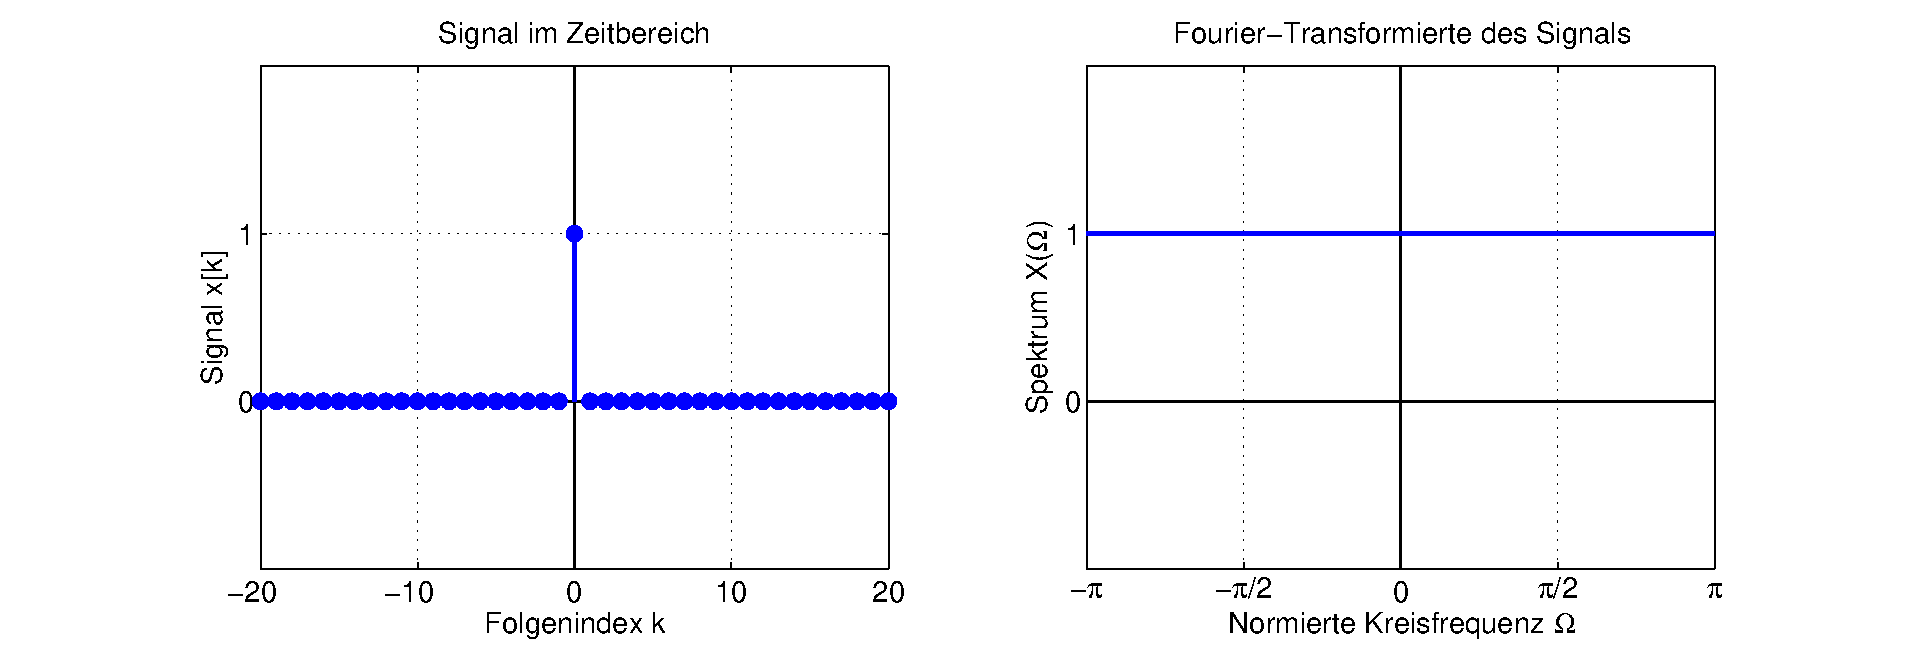
\includegraphics[width=1\textwidth]{Kapitel7/Bilder/image1.eps}}
  \caption{Impulsfolge und ihr Spektrum}
  \label{fig:FourierImpulsfolge}
\end{figure}

\noindent Wird der Impuls um k${}_{0}$ verschoben, \"{a}ndert sich die Fourier-Transformierte zu

\begin{equation}\label{eq:sevennineteen}
X\left(\Omega \right)=\sum _{k=-\infty }^{\infty }\delta \left[k-k_{0} \right]\cdot e^{-j\cdot \Omega \cdot k}  =e^{-j\cdot \Omega \cdot k_{0} } \cdot \sum _{k=-\infty }^{\infty }\delta \left[k-k_{0} \right] =e^{-j\cdot \Omega \cdot k_{0}}
\end{equation}

\noindent Eine Verschiebung des Impulses um k${}_{0}$ $\mathrm{>}$ 0 nach rechts f\"{u}hrt zu einer Multiplikation der Fourier-Transformierten mit z = e${}^{-j\cdot \Omega k_{0}}$. Diese Multiplikation \"{a}ndert die Phase des Spektrums, sein Betrag bleibt dagegen konstant.\bigskip

{\fontfamily{phv}\selectfont
\noindent\textbf{Kausale Rechteckfolge}}\smallskip

\noindent F\"{u}r die Rechteckfolge mit der Definition

\begin{equation}\label{eq:seventwenty}
x\left[k\right]=\sigma \left[k\right]-\sigma \left[k-K\right]
\end{equation}

\noindent wird die Summe in der Definitionsgleichung der Fourier-Transformation von Signalfolgen endlich. Mit der endlichen geometrischen Reihe 

\begin{equation}\label{eq:seventwentyone}
\sum _{k=0}^{K-1}q^{k}  =\frac{1-q^{K} }{1-q}
\end{equation}

\noindent ergibt sich die Fourier-Transformierte

\begin{equation}\label{eq:seventwentytwo}
X\left(\Omega \right)=\sum _{k=0}^{\infty }\left(\sigma \left[k\right]-\sigma \left[k-K\right]\right)\cdot e^{-j\cdot \Omega \cdot k}  =\sum _{k=0}^{K-1}e^{-j\cdot \Omega \cdot k}  =\frac{1-e^{-j\cdot \Omega \cdot K} }{1-e^{-j\cdot \Omega }}
\end{equation}

\noindent Zur \"{u}bersichtlicheren Trennung von Betrag und Phase werden aus Nenner und Z\"{a}hler Exponentialfunktionen ausgeklammert, sodass konjugiert komplexe Exponentialfunktionen entstehen. Sie werden zu einer Sinusfunktion zusammengefasst. 

\begin{equation}\label{eq:seventwentythree}
X\left(\Omega \right)=\frac{1-e^{-j\cdot \Omega \cdot K} }{1-e^{-j\cdot \Omega } } =\frac{e^{-j\cdot \frac{\Omega \cdot K}{2} } }{e^{-j\cdot \frac{\Omega }{2} } } \cdot \frac{\sin \left(\frac{K\cdot \Omega }{2} \right)}{\sin \left(\frac{\Omega }{2} \right)} =e^{-j\cdot \frac{\Omega \cdot \left(K-1\right)}{2} } \cdot \frac{\sin \left(\frac{K\cdot \Omega }{2} \right)}{\sin \left(\frac{\Omega }{2} \right)}
\end{equation}

\noindent Bild \ref{fig:FourierRechteckfolge} stellt die Rechteckfolge f\"{u}r K${}_{1}$ = 5 und K${}_{2}$ = 10 und den zugeh\"{o}rigen Betrag des Spektrums gegen\"{u}ber.

\begin{figure}[H]
  \centerline{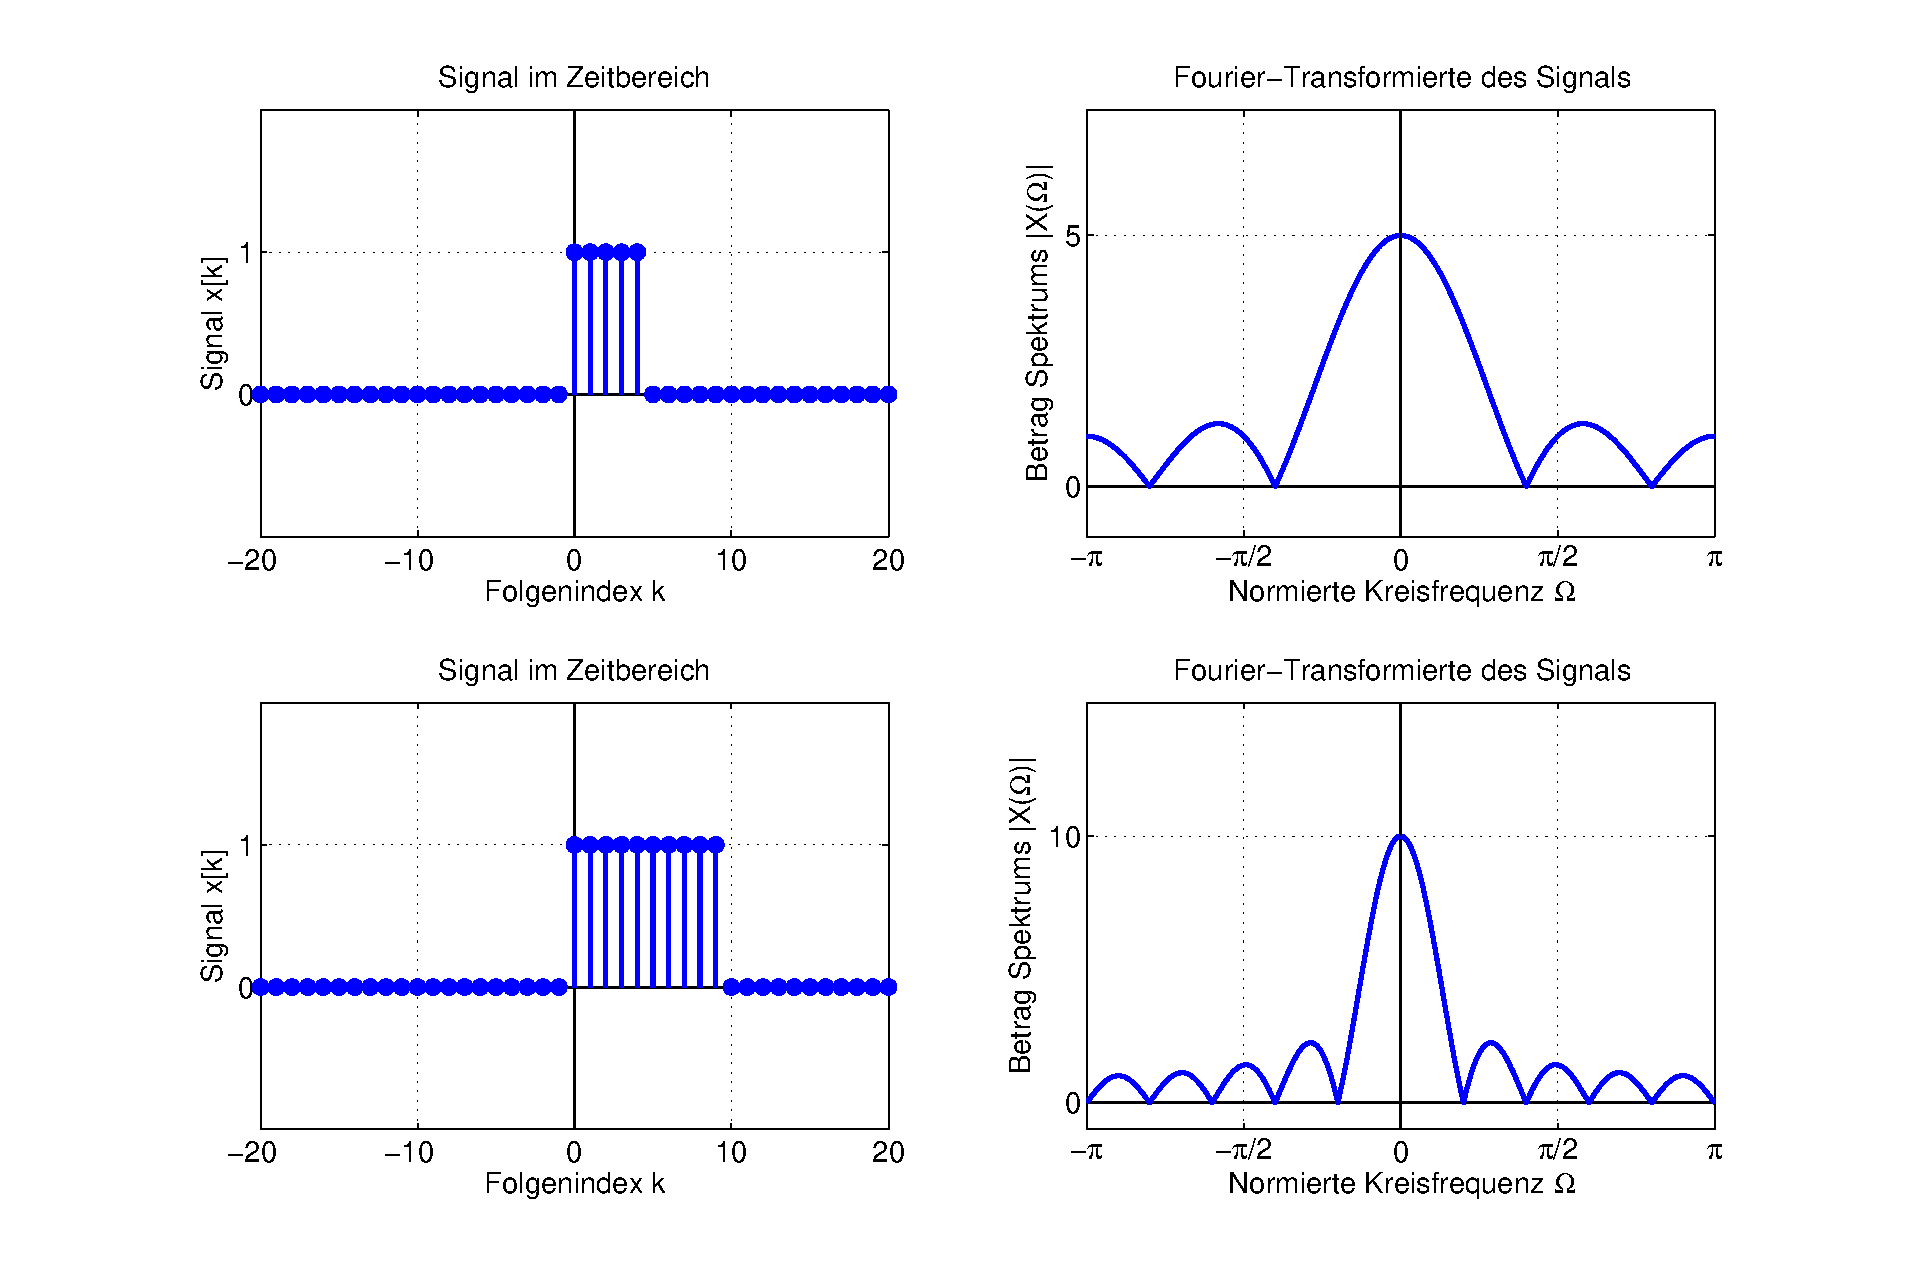
\includegraphics[width=1\textwidth]{Kapitel7/Bilder/image2.eps}}
  \caption{Rechteckfolge und Betrag ihres Spektrums f\"{u}r K${}_{1}$ = 5 und K${}_{2}$ = 10}
  \label{fig:FourierRechteckfolge}
\end{figure}

\noindent Die erste Nullstelle $\Omega_{0}$ des Spektrums liegt an der Stelle

\begin{equation}\label{eq:seventwentyfour}
\Omega _{0} =\frac{2\cdot \pi }{K}
\end{equation}

\noindent Wird diese Nullstelle als Ma{\ss} f\"{u}r die Breite des Spektrums angesehen, wird klar, dass das Spektrum mit sinkender Zahl K von Abtastwerten breiter wird. Im Extremfall liegt mit x[k] = $\delta$[k] ein einziger Abtastwert vor, und das Spektrum wird mit X($\Omega$) = 1 beliebig breit.\bigskip

{\fontfamily{phv}\selectfont
\noindent\textbf{Kausale Exponentialfolge}}\smallskip

\noindent Die kausale Potenzfolge ist definiert als 

\begin{equation}\label{eq:seventwentyfive}
x\left[k\right]=\lambda ^{k} \cdot \sigma \left[k\right]
\end{equation}

\noindent Ihre Fourier-Transformierte ergibt sich aus der Definitionsgleichung zu 

\begin{equation}\label{eq:seventwentysix}
X\left(\Omega \right)=\sum _{k=-\infty }^{\infty }\lambda ^{k} \cdot \sigma \left[k\right]\cdot e^{-j\cdot k\cdot \Omega }  =\sum _{k=0}^{\infty }\left(\lambda \cdot e^{-j\cdot \Omega } \right)^{k}
\end{equation}

\noindent Mit der Summationsformel f\"{u}r die geometrische Reihe 

\begin{equation}\label{eq:seventwentyseven}
\sum _{k=0}^{\infty }q^{k}=\frac{1}{1-q} \text{für} \left|{\rm q}\right|<1
\end{equation}

\noindent ergibt sich f\"{u}r {\textbar}$\lambda${\textbar} $\mathrm{<}$ 1 die Fourier-Transformierte

\begin{equation}\label{eq:seventwentyeight}
F\left\{\lambda ^{k} \cdot \sigma \left[k\right]\right\}=\sum _{k=0}^{\infty }\left(\lambda \cdot e^{-j\cdot \Omega } \right)^{k}  =\frac{1}{1-\lambda \cdot e^{-j\cdot \Omega } }
\end{equation}

\noindent Die Fourier-Transformierte der kausalen Exponentialfolge kann auf diese Art nur f\"{u}r {\textbar}$\lambda${\textbar} $\mathrm{<}$ 1 berechnet werden. F\"{u}r {\textbar}$\lambda${\textbar} $\mathrm{\ge}$ 1 existiert sie nicht. Bild \ref{fig:FourierEinseitigeExponentialfolge} stellt die kausale Exponentialfolgen mit $\lambda$ = 0.9 und $\lambda$ = - 0.9 sowie den Betrag ihrer Spektren dar.

\noindent Sowohl f\"{u}r $\lambda$ = 0.9, als auch f\"{u}r $\lambda$ = - 0.9 klingen die Signalfolgen x[k] ab. Wegen des negativen Vorzeichens handelt es sich bei $\lambda$ = - 0.9 um eine alternierende Folge. Durch den schnellen Signalwechsel bei der alternierenden Signalfolge besitzt das Spektrum der Exponentialfolge mit $\lambda$ = - 0.9 hohe Signalanteile bei den normierten Frequenzen $\Omega$ = $\mathrm{\pm}$ $\pi$, die der Abtastfrequenz $\mathrm{\pm}$ $\omega_{A}$/2 entsprechen. Im Gegensatz dazu weist das Spektrum der Exponentialfolge mit $\lambda$ = 0.9 wesentliche Spektralanteile an der Stelle $\Omega$ = 0 auf.

\begin{figure}[H]
  \centerline{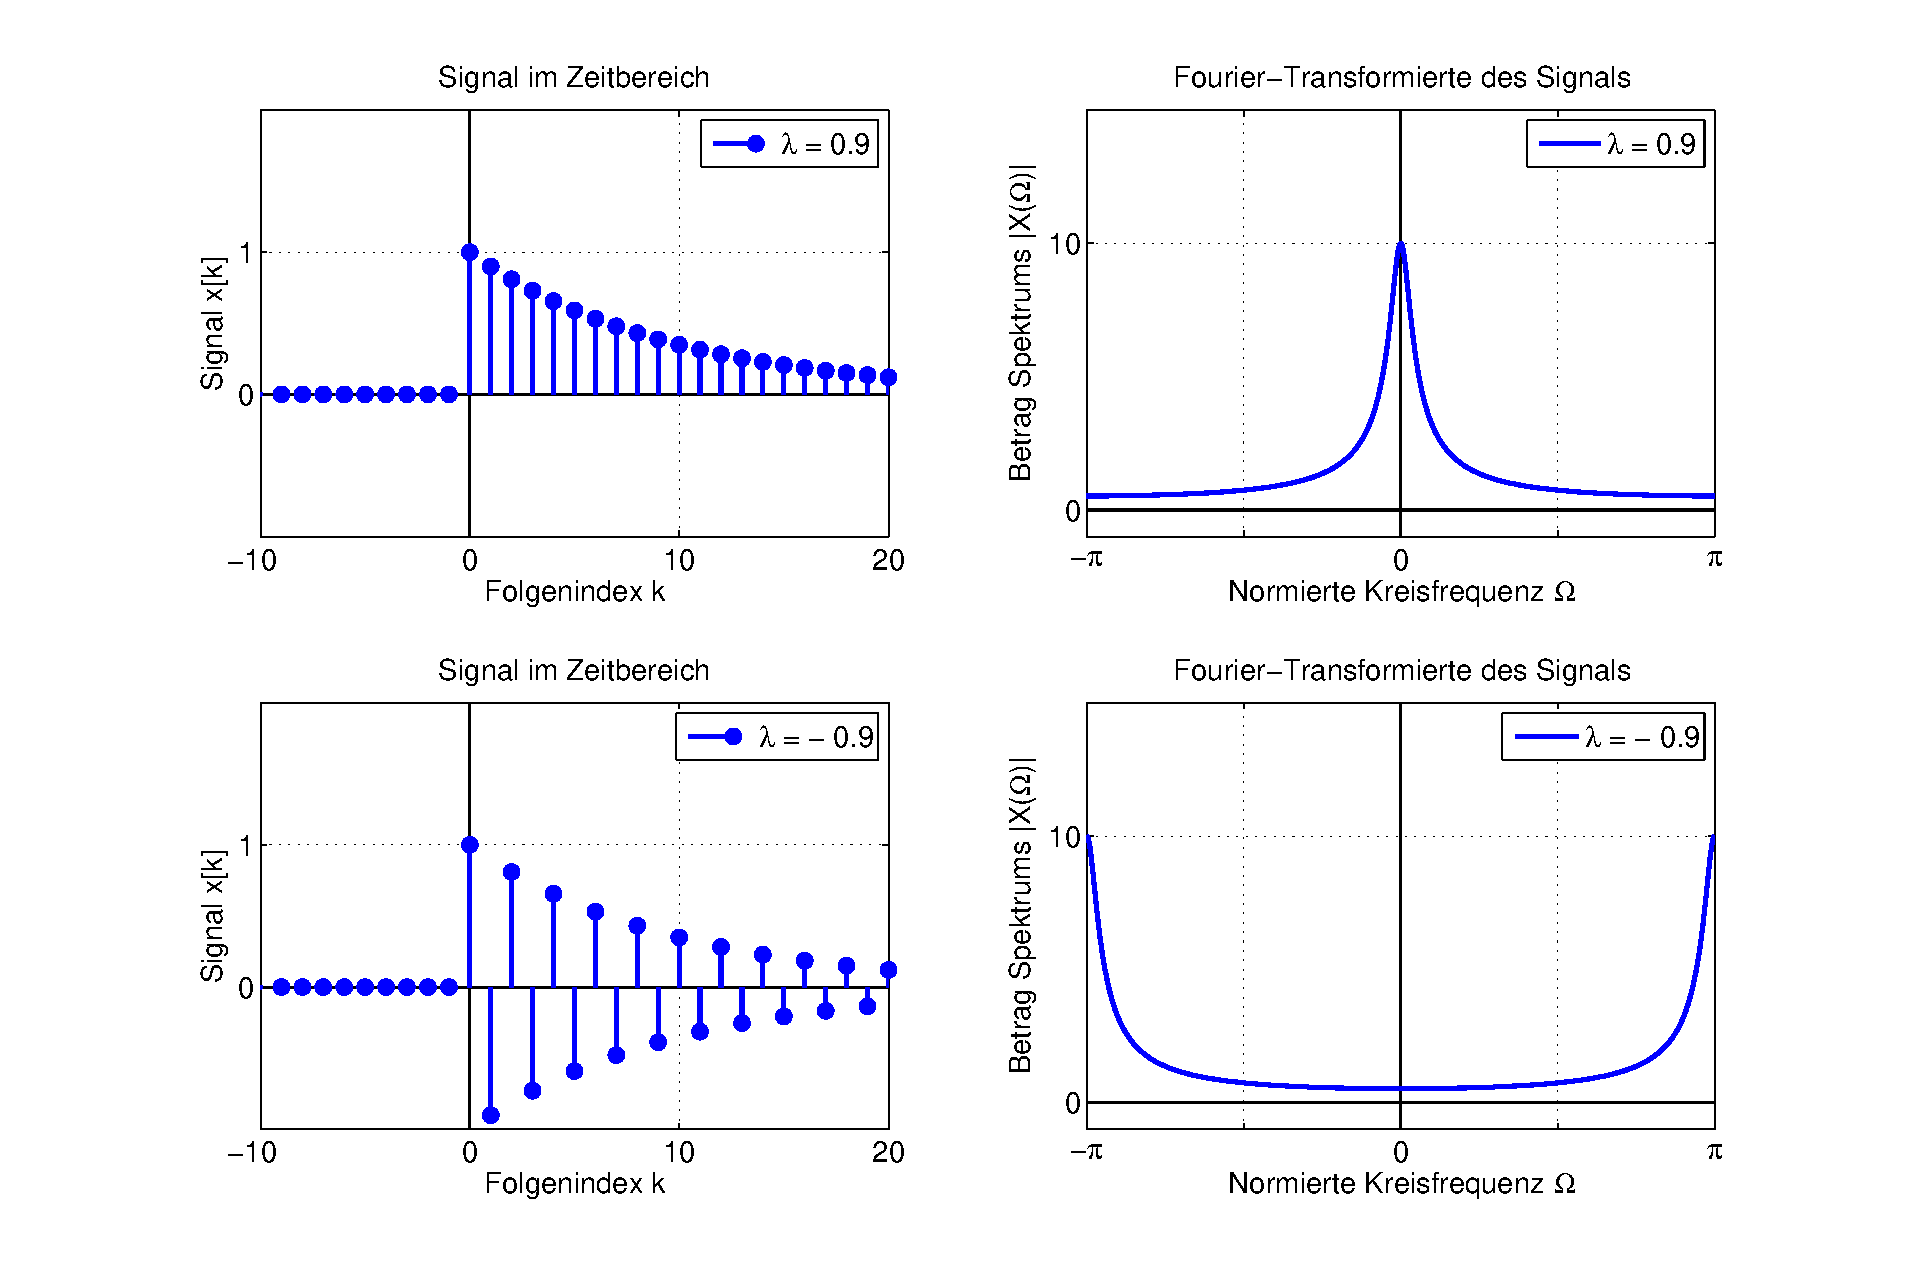
\includegraphics[width=1\textwidth]{Kapitel7/Bilder/image3.eps}}
  \caption{Kausale Exponentialfolge und Betrag ihres Spektrums f\"{u}r $\lambda$ = 0.9 und $\lambda$ = - 0.9}
  \label{fig:FourierEinseitigeExponentialfolge}
\end{figure}

\subsubsection{Existenz der Fourier-Transformation von Signalfolgen}

\noindent Bei der Berechnung der Fourier-Transformierten der kausalen Exponentialfolge ergibt sich die Bedingung {\textbar}$\lambda${\textbar} $\mathrm{<}$ 1 f\"{u}r die Konvergenz der zu berechnenden Reihe. Daraus resultiert die Frage, unter welchen Bedingungen die Fourier-Transformation von Signalfolgen konvergiert. Bei der Berechnung \"{u}ber die Definitionsgleichung wird die Reihe 

\begin{equation}\label{eq:seventwentynine}
X\left(\Omega \right)=\sum _{k=-\infty }^{\infty }x\left[k\right]\cdot e^{-j\cdot \Omega \cdot k}
\end{equation}

\noindent ausgewertet. Die Fourier-Transformierte existiert, wenn diese Reihe konvergiert. Eine hinreichende Bedingung f\"{u}r die Existenz der Fourier-Transformierten einer Folge ist ihre absolute Summierbarkeit.

\begin{equation}\label{eq:seventhirty}
\sum _{k=-\infty }^{\infty }\left|x\left[k\right]\right|<\infty
\end{equation}

\noindent Zwei Spezialf\"{a}lle werden diskutiert, kausale Signalfolgen und zeitlich begrenzte Signalfolgen.\bigskip

{\fontfamily{phv}\selectfont
\noindent\textbf{Kausale Signalfolgen}}\smallskip

\noindent Bei kausalen Signalfolgen kann die Konvergenzbedingung aus der geometrischen Reihe abgeleitet werden. Dabei wird ihre Konvergenz auf eine Betrachtung des Betrages von q reduziert. Um diesen Ansatz anwenden zu k\"{o}nnen, ist es wie bei der z-Transformation erforderlich, den Betrag der Folge x[k] mit Hilfe einer Exponentialfolge nach oben abzusch\"{a}tzen. 

\begin{equation}\label{eq:seventhirtyone}
\left|x\left[k\right]\right|\le X_{MAX} \cdot r^{k}
\end{equation}

\noindent Mit der Absch\"{a}tzung der Folge x[k] gilt f\"{u}r X($\Omega$)

\begin{equation}\label{eq:seventhirtytwo}
\left|X\left(\Omega \right)\right|=\left|\sum _{k=0}^{\infty }x\left[k\right]\cdot e^{-j\cdot \Omega \cdot k}  \right|\le \sum _{k=0}^{\infty }\left|x\left[k\right]\right|\cdot \left|e^{-j\cdot \Omega \cdot k} \right| \le \sum _{k=0}^{\infty }X_{MAX} \cdot r^{k}  =X_{MAX} \cdot \sum _{k=0}^{\infty }r^{k} 
\end{equation}

\noindent Damit existiert die Fourier-Transformierte, wenn f\"{u}r den Betrag von r gilt:

\begin{equation}\label{eq:seventhirtythree}
\left|r\right|<1
\end{equation}

\noindent Also kann die Fourier-Transformierte f\"{u}r alle kausalen Signale, deren z-Transformierte X(z) ausschlie{\ss}lich Pole innerhalb des Einheitskreises besitzt, \"{u}ber die Definitionsgleichung berechnet werden.\bigskip

{\fontfamily{phv}\selectfont
\noindent\textbf{Zeitlich begrenzte Signalfolgen}}\smallskip

\noindent Bei zeitlich begrenzten Signalfolgen mit endlicher Amplitude existiert immer eine Fourier-Transformierte. Zum Beweis wird die Definitionsgleichung der Fourier-Transformation nach oben abgesch\"{a}tzt.

\begin{equation}\label{eq:seventhirtyfour}
\left|X\left(\Omega \right)\right|=\left|\sum _{k=-\infty }^{\infty }x\left[k\right]\cdot e^{-j\cdot \Omega \cdot k}  \right|\le \sum _{k=-\infty }^{\infty }\left|x\left[k\right]\right| =\sum _{k=k_{1} }^{k_{2} }\left|x\left[k\right]\right|
\end{equation}

\noindent Da die Abtastwerte nur im Bereich k${}_{1}$ $\leq$ k $\leq$ k${}_{2}$ von null verschieden und ihre Werte begrenzt sind, ist die Summe endlich. 

\noindent Bei der Berechnung der Fourier-Transformierten von Leistungssignalen in Abschnitt 7.1.6 zeigt sich, dass die Bedingung der absoluten Summierbarkeit eine hinreichende, aber keine notwendige Bedingung ist. 

\subsubsection{Inverse Fourier-Transformation diskreter Folgen}

\noindent Das Spektrum einer Signalfolge X($\Omega$) ist eine in 2$\cdot\pi$ periodische Funktion. \"{A}hnlich wie bei periodischen Zeitsignalen kann diese Funktion mit Hilfe einer Reihe dargestellt werden. Es ergibt sich die Folge der Abtastwerte 

\begin{equation}\label{eq:seventhirtyfive}
x\left[k\right]=\frac{1}{2\cdot \pi } \cdot \int\limits _{-\pi }^{\pi }X\left(\Omega \right)\cdot e^{j\cdot \Omega \cdot k}d\Omega
\end{equation}

\noindent Als Beweis wird gezeigt, dass die Fourier-Transformation von Folgen und ihre R\"{u}cktransformation invers zueinander sind. Dazu wird die Gleichung f\"{u}r die Fourier-Transformation von Folgen in die Gleichung zur R\"{u}cktransformation eingesetzt. Als Ergebnis muss sich die Folge x[k] ergeben.

\begin{equation}\label{eq:seventhirtysix}
x\left[k\right]=\frac{1}{2\cdot \pi } \cdot \int\limits _{-\pi }^{\pi }X\left(\Omega \right)\cdot e^{j\cdot \Omega \cdot k} d\Omega  =\frac{1}{2\cdot \pi } \cdot \int _{-\pi }^{\pi }\left(\sum _{\kappa =-\infty }^{\infty }x\left[\kappa \right]\cdot e^{-j\cdot \Omega \cdot \kappa }  \right)\cdot e^{j\cdot \Omega \cdot k}d\Omega
\end{equation}

\noindent Zum Beweis wird die Reihenfolge von Summation und Integration vertauscht, und die beiden Exponentialfunktionen werden zusammengefasst.

\begin{equation}\label{eq:seventhirtyseven}
\begin{split}
x\left[k\right] & = \frac{1}{2\cdot \pi } \cdot \int\limits _{-\pi }^{\pi }\left(\sum _{\kappa =-\infty }^{\infty }x\left[\kappa \right]\cdot e^{-j\cdot \Omega \cdot \kappa }  \right)\cdot e^{j\cdot \Omega \cdot k} d\Omega  =\sum _{\kappa =-\infty }^{\infty }x\left[\kappa \right]\cdot \frac{1}{2\cdot \pi } \cdot \int\limits _{-\pi }^{\pi }e^{-j\cdot \Omega \cdot \kappa } \cdot e^{j\cdot \Omega \cdot k} d\Omega \\
&=\sum _{\kappa =-\infty }^{\infty }x\left[\kappa \right]\cdot \frac{1}{2\cdot \pi } \cdot \int\limits _{-\pi }^{\pi } e^{j\cdot \Omega \cdot (k-\kappa)} d\Omega
\end{split}
\end{equation}

\noindent Das Integral der komplexen Exponentialfunktion \"{u}ber eine volle Periode ist null. Nur f\"{u}r k = $\kappaup$ wird aus der komplexen Exponentialfunktion die Zahl eins. Das Ergebnis kann mit der Impulsfolge dargestellt werden. Mit der Ausblendeigenschaft der Impulsfolge ergibt sich 

\begin{equation}\label{eq:seventhirtyeight}
\sum _{\kappa =-\infty }^{\infty }x\left[\kappa \right]\cdot \frac{1}{2\cdot \pi } \cdot \int\limits _{-\pi }^{\pi }e^{j\cdot \Omega \cdot \left(k-\kappa \right)} d\Omega=\sum _{\kappa =-\infty }^{\infty }x\left[\kappa \right]\cdot \delta [k-\kappa ] =x\left[k\right]
\end{equation}

\noindent Der Umgang mit der R\"{u}cktransformation wird an einem Beispiel vertieft.\bigskip

\noindent
\colorbox{lightgray}{%
\arrayrulecolor{white}%
\renewcommand\arraystretch{0.6}%
\begin{tabular}{ wl{16.5cm} }
{\fontfamily{phv}\selectfont{Beispiel: Inverse Fourier-Transformation diskreter Folgen}}
\end{tabular}%
}\medskip

\noindent Zu einem rechteckf\"{o}rmigen Spektrum der Form

\begin{equation}\label{eq:seventhirtynine}
X\left(\Omega \right)=\sigma \left(\Omega +\frac{\pi }{2} \right)-\sigma \left(\Omega -\frac{\pi }{2} \right)
\end{equation}

\noindent soll die zugeh\"{o}rige Signalfolge x[k] berechnet werden. Dazu wird die Gleichung zur R\"{u}cktransformation verwendet. F\"{u}r k $\mathrm{\neq}$ 0 ergibt sich

\begin{equation}\label{eq:sevenfourty}
\begin{split}
x\left[k\right] & =\frac{1}{2\cdot \pi } \cdot \int\limits _{-\pi }^{\pi }X\left(\Omega \right)\cdot e^{j\cdot \Omega \cdot k} {\rm \; }d\Omega  =\frac{1}{2\cdot \pi } \cdot \int\limits _{-\pi /2}^{\pi /2}e^{j\cdot \Omega \cdot k} {\rm \; }d\Omega  =\frac{1}{2\cdot \pi } \cdot \left. \frac{1}{j\cdot k} \cdot e^{j\cdot \Omega \cdot k} \right|_{-\pi /2}^{\pi /2} \\
&=\frac{1}{2\cdot \pi } \cdot \frac{1}{j\cdot k}\cdot 2\cdot j \cdot sin\left(\frac{\pi}{2}\cdot k\right)= \frac{1}{k\cdot \pi}\cdot sin\left(\frac{\pi}{2}\cdot k\right)
\end{split}
\end{equation}

\noindent F\"{u}r k = 0 errechnet sich der Wert x[0] zu

\begin{equation}\label{eq:sevenfourtyone}
x\left[0\right]=\frac{1}{2\cdot \pi } \cdot \int\limits _{-\pi }^{\pi }X\left(e^{j\cdot \Omega } \right)\cdot e^{j\cdot \Omega \cdot 0} d\Omega  =\frac{1}{2\cdot \pi } \cdot \int\limits _{-\pi /2}^{\pi /2}1 d\Omega  =\frac{\pi }{2\cdot \pi} =\frac{1}{2}
\end{equation}

\noindent Wie bei zeitkontinuierlichen Signalen kann aus dem Spektrum X($\Omega$) eine eindeutige Signalfolge x[k] berechnet werden. Bild \ref{fig:FourierRechteckSpektrum} stellt die Signalfolge und ihre Fourier-Transformierte gegen\"{u}ber.

\begin{figure}[H]
  \centerline{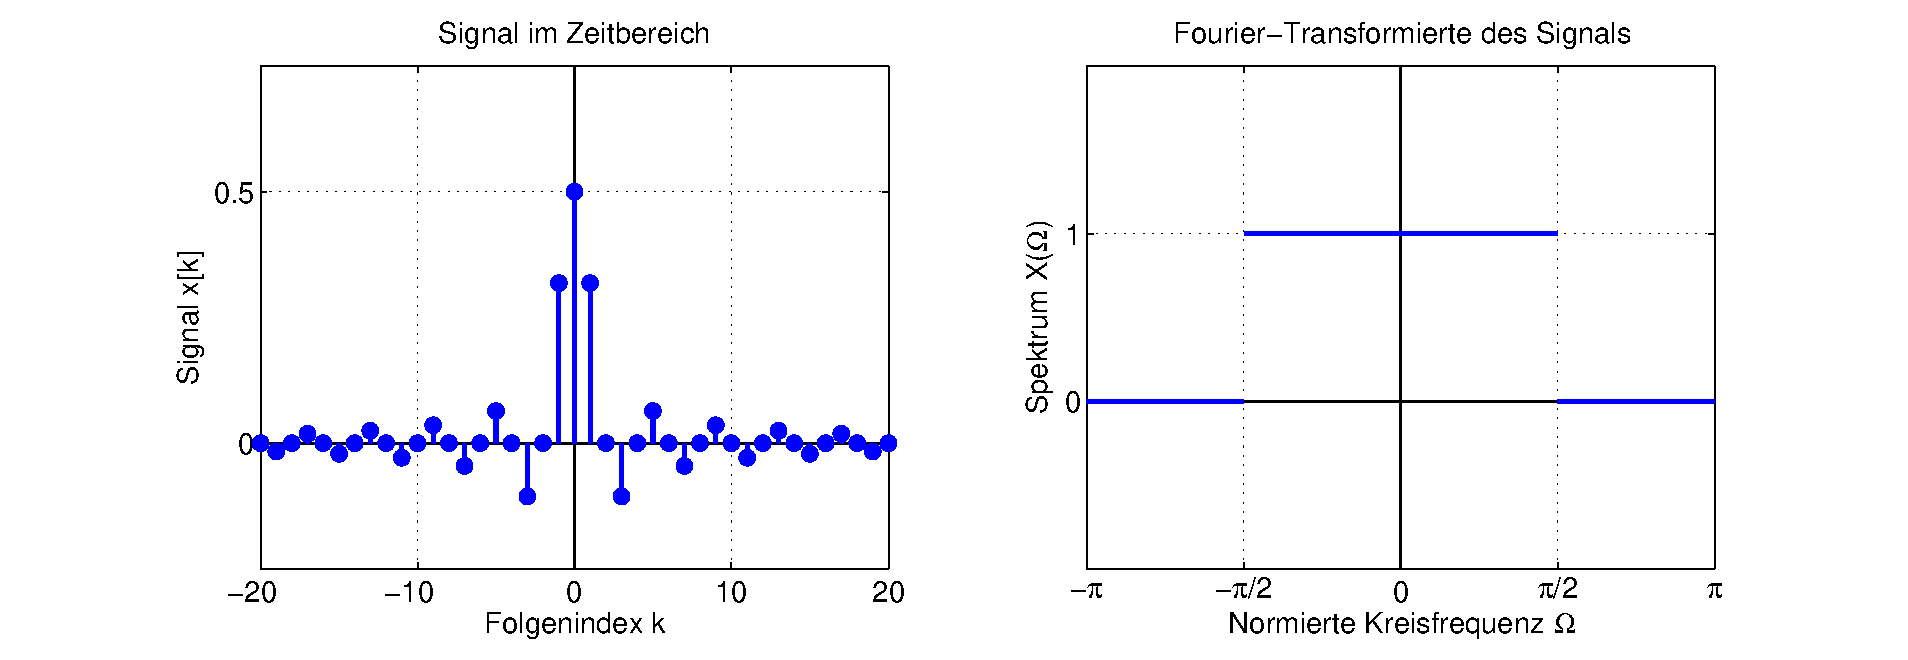
\includegraphics[width=1\textwidth]{Kapitel7/Bilder/image4.eps}}
  \caption{Signalfolge und ihr rechteckf\"{o}rmiges Spektrum}
  \label{fig:FourierRechteckSpektrum}
\end{figure}

\subsubsection{Fourier-Transformierte von Leistungssignalfolgen}

\noindent In Abschnitt 7.1.4 wird eine hinreichende Bedingung f\"{u}r die Existenz der Fourier-Transformierten einer Signalfolge hergeleitet und diskutiert. Es zeigt sich, dass die absolute Summierbarkeit eine hinreichende Bedingung ist. Aus diesem Grund existiert f\"{u}r Energiesignalfolgen immer eine Fourier-Transformierte. Aber auch f\"{u}r Leistungssignalfolgen l\"{a}sst sich eine Fourier-Transformierte bestimmen. \"{A}hnlich wie im zeitkontinuierlichen Bereich wird dazu die Impulsfunktion im Frequenzbereich verwendet. Da bei zeitdiskreten Signalen das Spektrum periodisch in 2$\cdot\pi$ ist, wird die Signalfolge x[k] zu dem Spektrum

\begin{equation}\label{eq:sevenfourtytwo}
X\left(\Omega \right)=\sum _{\nu =-\infty }^{\infty }\delta \left(\Omega -2\cdot \pi \cdot \nu \right)
\end{equation}

\noindent berechnet. Mit der Definitionsgleichung der inversen Fourier-Transformation von Signalfolgen ergibt sich

\begin{equation}\label{eq:sevenfourtythree}
x\left[k\right]=\frac{1}{2\cdot \pi} \cdot \int\limits _{-\pi }^{\pi }\sum _{\nu =-\infty }^{\infty }\delta \left(\Omega -2\cdot \pi \cdot \nu \right) \cdot e^{j\cdot \Omega \cdot k} d\Omega
\end{equation}

\noindent In dem Bereich von - $\pi$ $\leq$ $\Omega$ $\leq$ $\pi$ liegt nur der Impuls an der Stelle $\Omega$ = 0. Damit ergibt sich mit der Ausblendeigenschaft der Impulsfunktion

\begin{equation}\label{eq:sevenfourtyfour}
x\left[k\right]=\frac{1}{2\cdot \pi } \cdot \int\limits _{-\pi }^{\pi }\delta \left(\Omega \right)\cdot e^{j\cdot \Omega \cdot k} d\Omega  =\frac{1}{2\cdot \pi }
\end{equation}

\noindent Diese Folge x[k] ist nach den Ausf\"{u}hrungen in Abschnitt 3.1.3 keine Energiesignalfolge, trotzdem besitzt sie eine Fourier-Transformierte. Bild \ref{fig:FourierEinsfolge} stellt die Einsfolge und ihre Fourier-Transformierte gegen\"{u}ber.

\begin{figure}[H]
  \centerline{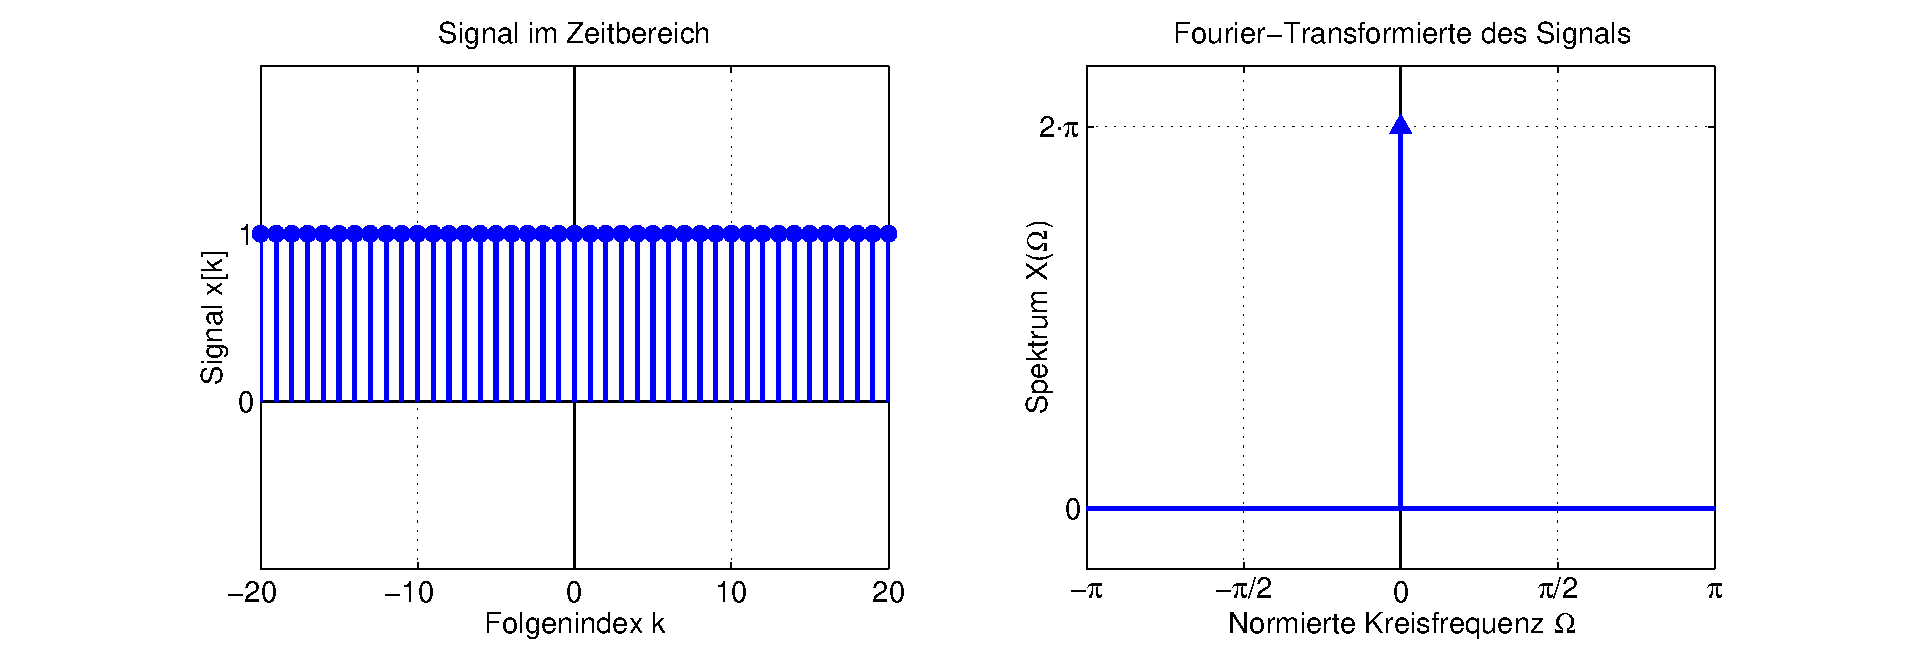
\includegraphics[width=1\textwidth]{Kapitel7/Bilder/image5.eps}}
  \caption{Einsfolge und ihr Spektrum}
  \label{fig:FourierEinsfolge}
\end{figure}

\noindent Mit den Rechenregeln zur Fourier-Transformation von Signalfolgen lassen sich mit dieser Korrespondenz weitere Korrespondenzen herleiten. \bigskip

\noindent
\colorbox{lightgray}{%
\arrayrulecolor{white}%
\renewcommand\arraystretch{0.6}%
\begin{tabular}{ wl{16.5cm} }
{\fontfamily{phv}\selectfont{Beispiel: Korrespondenz der Kosinusfolge}}
\end{tabular}%
}\medskip

\noindent Bei der zeitkontinuierlichen Fourier-Transformation kann das Spektrum einer harmonischen Funktion \"{u}ber die R\"{u}cktransformation bestimmt werden. In diesem Beispiel wird diese Idee f\"{u}r Folgen aufgegriffen. Es wird die zu dem Spektrum 

\begin{equation}\label{eq:sevenfourtyfive}
X\left(\Omega \right)=\sum _{\nu =-\infty }^{\infty }\delta \left(\Omega +\Omega _{0} +2\cdot \pi \cdot \nu \right)+\delta \left(\Omega -\Omega _{0} +2\cdot \pi \cdot \nu \right)
\end{equation}

\noindent geh\"{o}rige Signalfolge x[k] berechnet. Dabei liegt $\Omega_{0}$ in dem Bereich 0 $\mathrm{<}$ $\Omega_{0}$ $\mathrm{<}$ $\pi$. F\"{u}r die Berechnung der entsprechenden Signalfolge x[k] wird die Gleichung zur R\"{u}cktransformation verwendet und der Ausdruck in zwei separate Integrale aufgeteilt.

\begin{equation}\label{eq:sevenfourtysix}
\begin{split}
x\left[k\right] &=\frac{1}{2\cdot \pi } \cdot \int\limits _{-\pi }^{\pi }X\left(\Omega \right)\cdot e^{j\cdot \Omega \cdot k}d\Omega  =\frac{1}{2\cdot \pi } \cdot \int\limits _{-\pi }^{\pi }\left(\delta \left(\Omega +\Omega _{0} \right)+\delta \left(\Omega -\Omega _{0} \right)\right)\cdot e^{j\cdot \Omega \cdot k}d\Omega\\ 
&=\frac{1}{2\cdot \pi} \cdot\int\limits _{-\pi }^{\pi }\delta \left(\Omega +\Omega _{0} \right)\cdot e^{j\cdot \Omega \cdot k}d\Omega+\frac{1}{2\cdot \pi} \cdot\int\limits _{-\pi }^{\pi }\delta \left(\Omega -\Omega _{0} \right)\cdot e^{j\cdot \Omega \cdot k}d\Omega
\end{split}
\end{equation}

\noindent Jedes Integral kann mit der Ausblendeigenschaft der Impulsfunktion gel\"{o}st werden.

\begin{equation}\label{eq:sevenfourtyseven}
\begin{split}
x\left[k\right] &=\frac{1}{2\cdot \pi } \cdot e^{-j\cdot \Omega _{0} \cdot k} \cdot \int\limits _{-\pi }^{\pi }\delta \left(\Omega +\Omega _{0} \right)d\Omega  +\frac{1}{2\cdot \pi } \cdot e^{j\cdot \Omega _{0} \cdot k} \cdot \int\limits _{-\pi }^{\pi }\delta \left(\Omega -\Omega _{0} \right)d\Omega \\
&=\frac{1}{2\cdot \pi } \cdot ( e^{j\cdot \Omega _{0} \cdot k}+e^{-j\cdot \Omega _{0} \cdot k})=\frac{2}{2\cdot \pi } \cdot \cos(\Omega _{0} \cdot k)=\frac{1}{\pi}\cdot \cos(k\cdot\Omega_{0})
\end{split}
\end{equation}

\noindent Damit ergibt sich die Korrespondenz zur Kosinusfolge zu

\begin{equation}\label{eq:sevenfourtyeight}
F\left\{\cos \left(k\cdot \Omega _{0} \right)\right\}=\pi \cdot \sum _{\nu =-\infty }^{\infty }\delta \left(\Omega +\Omega _{0} +2\cdot \pi \cdot \nu \right)+\delta \left(\Omega -\Omega _{0} +2\cdot \pi \cdot \nu \right)
\end{equation}

\noindent Bild \ref{fig:FourierKosinusfolge} stellt eine Kosinusfolge mit $\Omega_{0}$ = $\piup$/3 und ihre Fourier-Transformierten dar.

\begin{figure}[H]
  \centerline{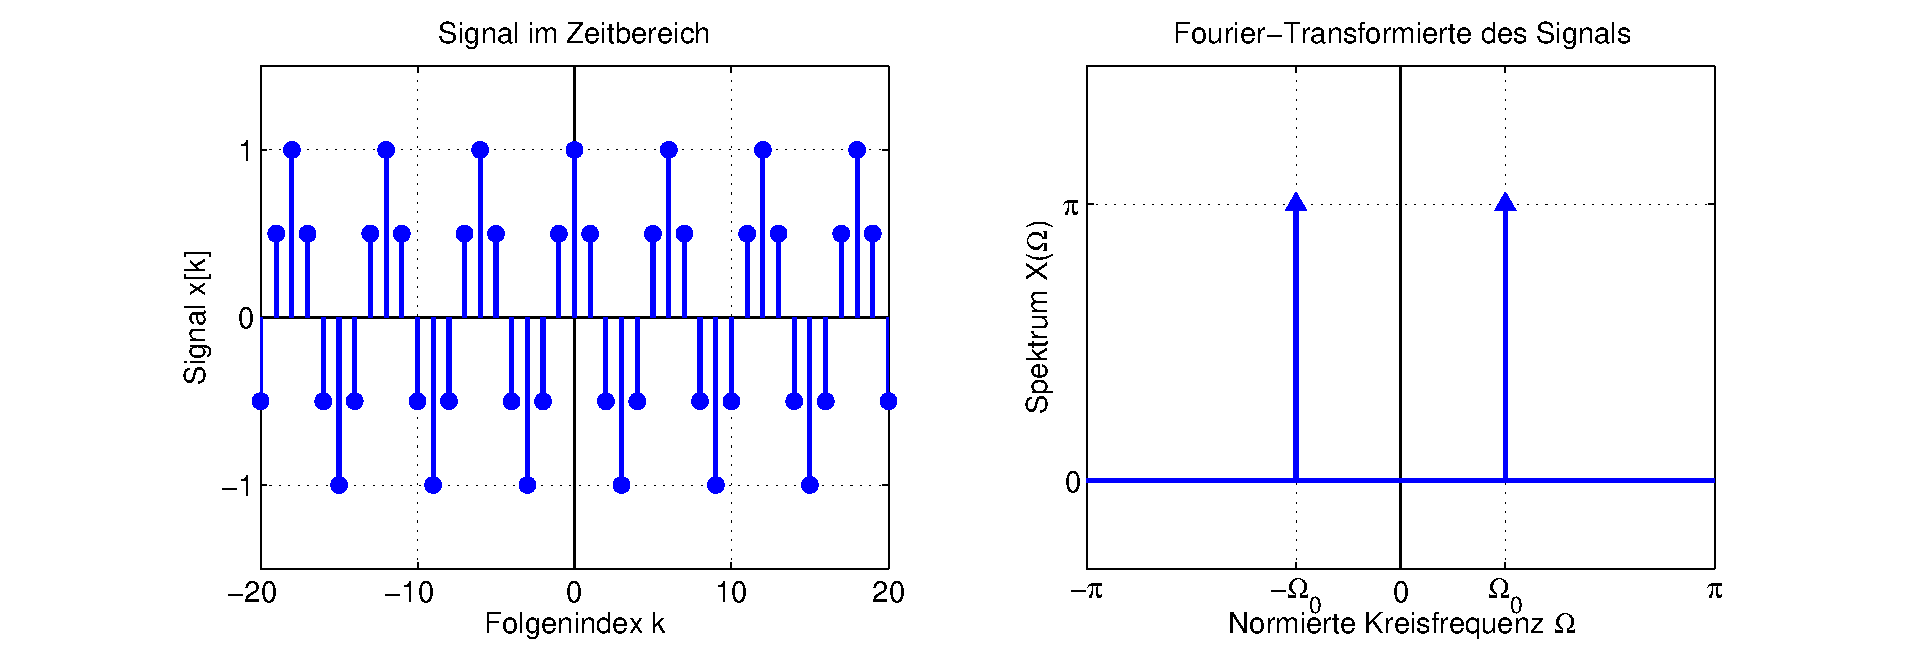
\includegraphics[width=1\textwidth]{Kapitel7/Bilder/image6.eps}}
  \caption{Kosinusfolge und ihr Spektrum}
  \label{fig:FourierKosinusfolge}
\end{figure}

\noindent Auf demselben Weg kann die Fourier-Transformierte der Sinusfolge hergeleitet werden.

\subsubsection{Symmetrieeigenschaften der Fourier-Transformation von Signalfolgen}

\noindent Bei der Anwendung der Fourier-Transformation k\"{o}nnen Symmetriebedingungen genutzt werden, um aus existierenden Korrespondenzen weitere Korrespondenzen abzuleiten. Insbesondere bei reellen Zahlenfolgen k\"{o}nnen die Symmetriebedingungen f\"{u}r eine schnelle Plausibilisierung von Ergebnissen verwendet werden. \newline
\noindent Im Folgenden werden die wesentlichen Symmetrieeigenschaften f\"{u}r komplexe und reelle Signalfolgen zusammengefasst. Weitere Symmetrieregeln und ihre Herleitung sind in [Oppe04] zu finden. Dabei wird davon ausgegangen, dass zur Signalfolge x[k] das Spektrum X($\Omega$) geh\"{o}rt.

\begin{table}[H]
\setlength{\arrayrulewidth}{.1em}
\caption{Symmetrieregeln der Fourier-Transformation f\"{u}r komplexe Signalfolgen}
\setlength{\fboxsep}{0pt}%
\colorbox{lightgray}{%
\arrayrulecolor{white}%
\begin{tabular}{| c | c |}
\hline
\parbox[c][0.35in][c]{3.3in}{\smallskip\centering\textbf{\fontfamily{phv}\selectfont{Folge x[k]}}} & 
\parbox[c][0.35in][c]{3.3in}{\smallskip\centering\textbf{\fontfamily{phv}\selectfont{Fourier-Transformierte X($\Omega$)}}}\\ \hline

\parbox[c][0.4in][c]{3.3in}{\centering{\fontfamily{phv}\selectfont{Gerade Folge}}} & 
\parbox[c][0.4in][c]{3.3in}{\centering{\fontfamily{phv}\selectfont{Reelles Spektrum $X(\Omega)$}}}\\ \hline

\parbox[c][0.4in][c]{3.3in}{\centering{\fontfamily{phv}\selectfont{Ungerade Folge}}} & 
\parbox[c][0.4in][c]{3.3in}{\centering{\fontfamily{phv}\selectfont{Imagin\"{a}res Spektrum $X(\Omega)$}}}\\ \hline

\parbox[c][0.4in][c]{3.3in}{\centering{\fontfamily{phv}\selectfont{Konjugiert komplexe Folge x*[k]}}} & 
\parbox[c][0.4in][c]{3.3in}{\centering{$X*(- \Omega)$}}\\ \hline

\parbox[c][0.4in][c]{3.3in}{\centering{\fontfamily{phv}\selectfont{Gespiegelte konjugiert komplexe Folge x*[- k]}}} & 
\parbox[c][0.4in][c]{3.3in}{\centering{$X*(\Omega)$}}\\ \hline

\end{tabular}%
}
\label{tab:seventwo}
\end{table}


\begin{table}[H]
\setlength{\arrayrulewidth}{.1em}
\caption{Symmetrieregeln der Fourier-Transformation f\"{u}r reelle Signalfolgen x[k]}
\setlength{\fboxsep}{0pt}%
\colorbox{lightgray}{%
\arrayrulecolor{white}%
\begin{tabular}{| c | c |}
\hline
\parbox[c][0.35in][c]{3.3in}{\smallskip\centering\textbf{\fontfamily{phv}\selectfont{Regel}}} & 
\parbox[c][0.35in][c]{3.3in}{\smallskip\centering\textbf{\fontfamily{phv}\selectfont{Anmerkung}}}\\ \hline

\parbox[c][0.4in][c]{3.3in}{\centering{X($\Omega$) = X*(- $\Omega$)}} & 
\parbox[c][0.4in][c]{3.3in}{\centering{Fourier-Transformierte einer reellen Folge ist konjugiert symmetrisch}}\\ \hline

\parbox[c][0.4in][c]{3.3in}{\centering{X${}_{R}$($\Omega$) = X${}_{R}$(- $\Omega$)}} &
\parbox[c][0.4in][c]{3.3in}{\centering{Realteil der Fourier-Transformierten ist gerade}}\\ \hline

\parbox[c][0.4in][c]{3.3in}{\centering{X${}_{I}$($\Omega$) = - X${}_{I}$(- $\Omega$)}} & 
\parbox[c][0.4in][c]{3.3in}{\centering{Imagin\"{a}rteil der Fourier-Transformierten ist ungerade}}\\ \hline

\parbox[c][0.4in][c]{3.3in}{\centering{{\textbar}X($\Omega$){\textbar} = {\textbar}X(- $\Omega$){\textbar}}} & 
\parbox[c][0.4in][c]{3.3in}{\centering{Betrag der Fourier-Transformierten ist gerade}}\\ \hline

\parbox[c][0.4in][c]{3.3in}{\centering{$\varphi$($\Omega$) = - $\varphi$(- $\Omega$)}} & 
\parbox[c][0.4in][c]{3.3in}{\centering{Phase der Fourier-Transformierten ist ungerade}}\\ \hline

\end{tabular}%
}
\label{tab:seventhree}
\end{table}

\noindent
\colorbox{lightgray}{%
\arrayrulecolor{white}%
\renewcommand\arraystretch{0.6}%
\begin{tabular}{ wl{16.5cm} }
{\fontfamily{phv}\selectfont{Beispiel: Fourier-Transformierten der kausalen Exponentialfolge}}
\end{tabular}%
}\medskip

\noindent Es wird die Fourier-Transformierte der kausalen Exponentialfolge

\begin{equation}\label{eq:sevenfourtynine}
x\left[k\right]=\lambda ^{k} \cdot \sigma \left[k\right]
\end{equation}

\noindent diskutiert. Das Spektrum der kausalen Exponentialfolge berechnet sich zu

\begin{equation}\label{eq:sevenfifty}
X\left(\Omega \right)=\frac{1}{1-\lambda \cdot e^{-j\cdot \Omega } } =\frac{1}{1-\lambda \cdot \cos \left(\Omega \right)-j\cdot \lambda \cdot \sin \left(\Omega \right)}
\end{equation}

\noindent Die konjugiert symmetrische Fourier-Transformierte ergibt sich zu

\begin{equation}\label{eq:sevenfiftyone}
X^{*} \left(-\Omega \right)=\frac{1}{1-\lambda \cdot \cos \left(-\Omega \right)+j\cdot \lambda \cdot \sin \left(-\Omega \right)} =\frac{1}{1-\lambda \cdot \cos \left(\Omega \right)-j\cdot \lambda \cdot \sin \left(\Omega \right)}
\end{equation}

\noindent Beide Transformierten stimmen erwartungsgem\"{a}{\ss} \"{u}berein. Die Spektren der beiden Folgen sind in Bild 7.7 sowohl als Real- und Imagin\"{a}rteil, als auch als Betrag und Phase dargestellt.

\begin{figure}[H]
  \centerline{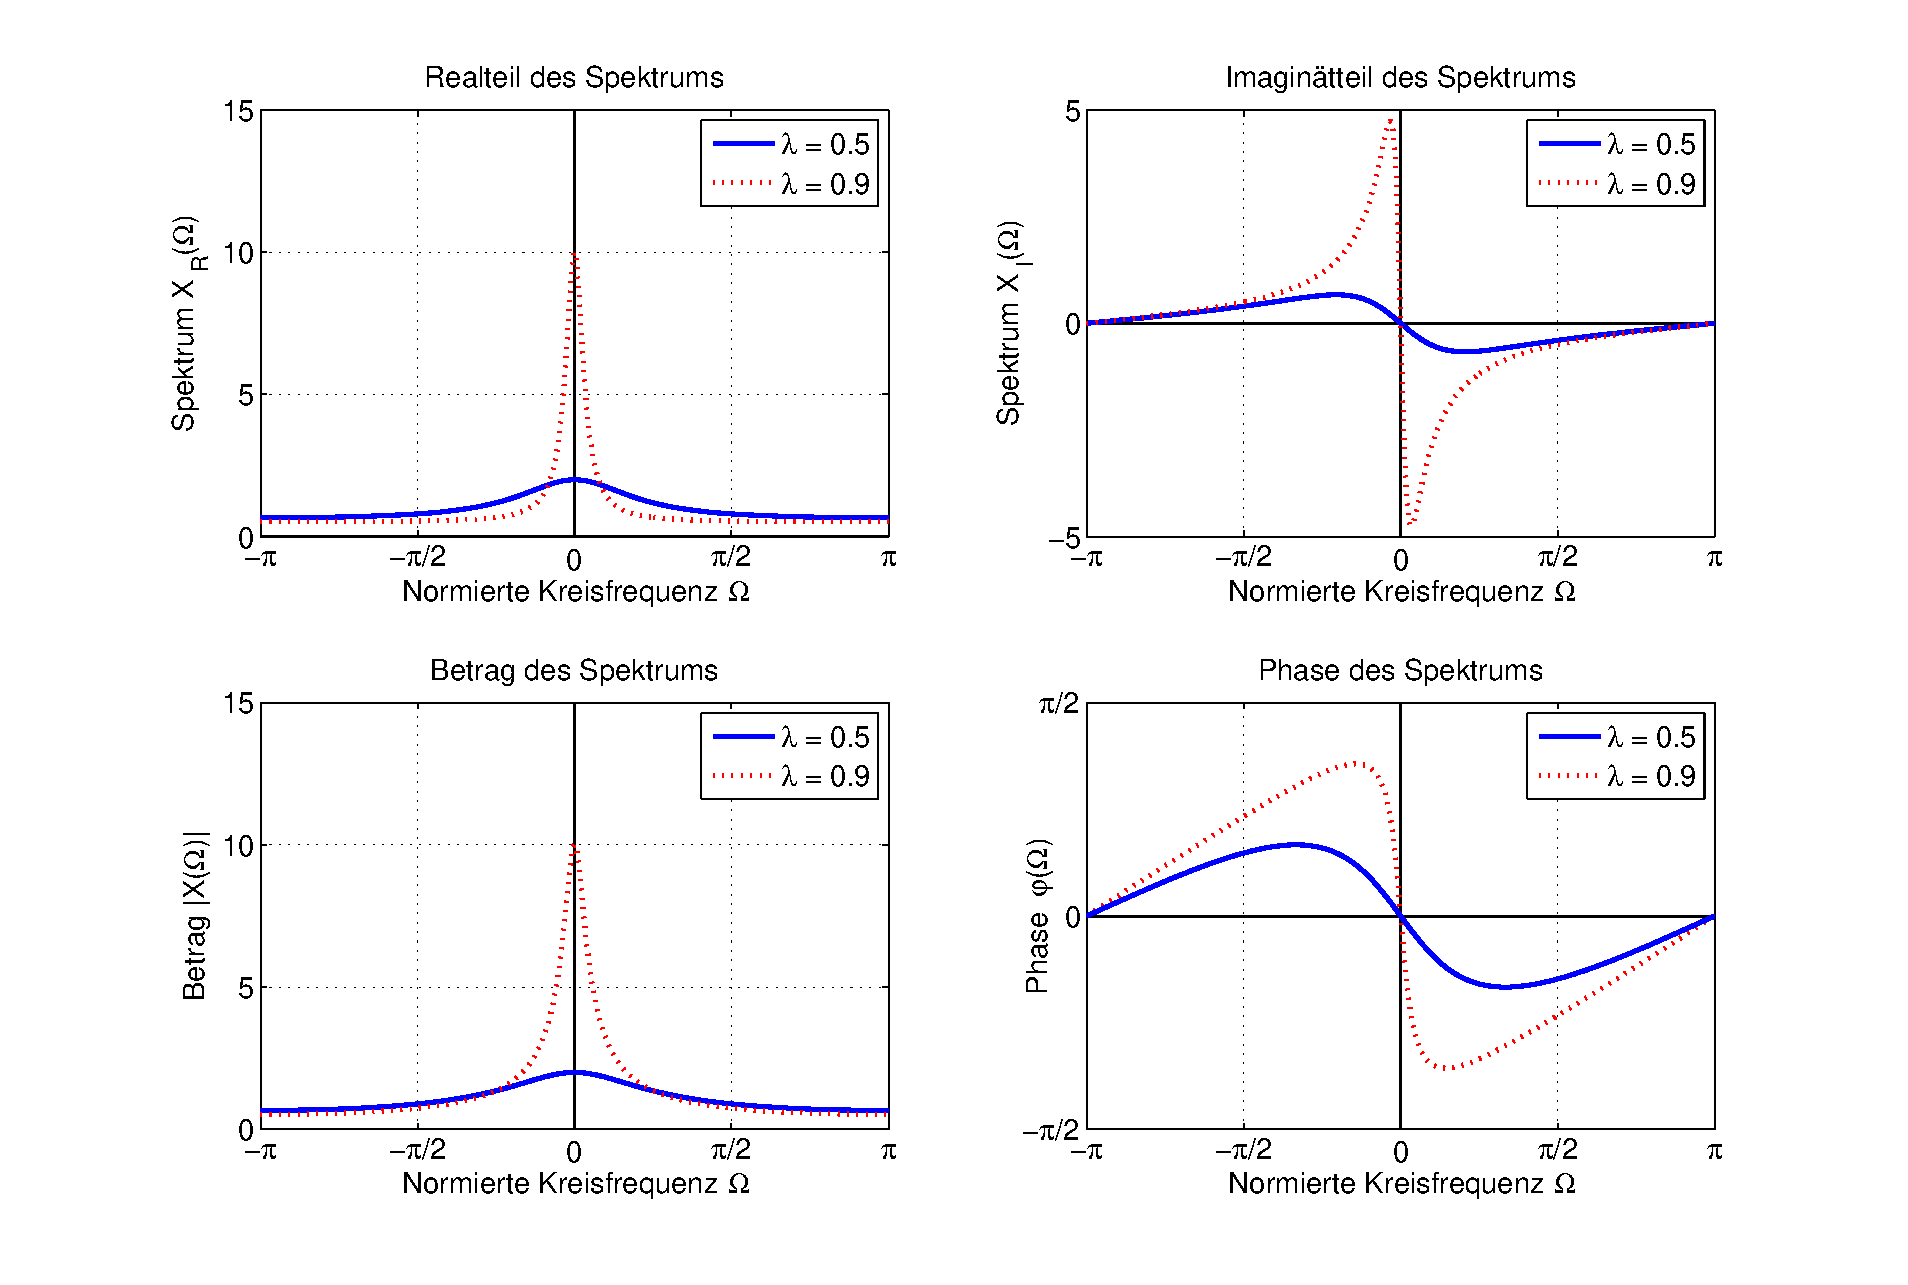
\includegraphics[width=1\textwidth]{Kapitel7/Bilder/image7.eps}}
  \caption{Spektren der kausalen Exponentialfolgen mit $\lambda$ = 0.5 und $\lambda$ = 0.9}
  \label{fig:EinseitigeExponentialfolgeSymmetrie}
\end{figure}

\noindent Der Realteil des Spektrums ist gerade, der Imagin\"{a}rteil ist ungerade. Der Betrag des Spektrums ist gerade, die Phase ungerade. Damit entsprechen die Symmetrien den in Tabelle \ref{tab:seventhree} dargestellten Symmetrieregeln.

\clearpage

\subsection{Rechenregeln der Fourier-Transformation von Signalfolgen}

\noindent Wie andere Transformationen besitzt die Fourier-Transformation von Signalfolgen Rechenregeln, die die Berechnung weiterer Korrespondenzen vereinfachen. Die Regeln werden im Folgenden hergeleitet und jeweils an einem Beispiel verdeutlicht. Sie entsprechen weitgehend den Rechenregeln f\"{u}r die Fourier-Transformation zeitkontinuierlicher Signale. Am Ende dieses Abschnittes sind alle Rechenregeln in einer \"{U}bersicht zusammengestellt.

\subsubsection{Linearit\"{a}t}

\noindent Wie die \"{u}brigen Integraltransformationen ist auch die Fourier-Transformation von Signalfolgen eine lineare Transformation. Durch Einsetzen in die Definitionsgleichung ergibt sich

\begin{equation}\label{eq:sevenfiftytwo}
F\left\{\nu _{1} \cdot x_{1} \left[k\right]+\nu _{2} \cdot x_{2} \left[k\right]\right\}=\sum _{k=-\infty }^{\infty }\left(\nu _{2} \cdot x_{1} \left[k\right]+\nu _{2} \cdot x_{2} \left[k\right]\right)\cdot e^{-j\cdot \Omega \cdot k}
\end{equation}

\noindent Im Fall absolut summierbarer Reihen besitzen beide Folgen x${}_{1}$[k] und x${}_{2}$[k] eigene Fourier-Transformierte X${}_{1}$($\Omega$) und X${}_{2}$($\Omega$). In dem Fall gilt das Distributivgesetz

\begin{equation}\label{eq:sevenfiftythree}
\begin{split}
\sum _{k=-\infty }^{\infty }\left(\nu _{1} \cdot x_{1} \left[k\right]+\nu _{2} \cdot x_{2} \left[k\right]\right)\cdot e^{-j\cdot k\cdot \Omega} & = \sum _{k=-\infty }^{\infty }\nu _{1} \cdot x_{1} \left[k\right]\cdot e^{-j\cdot \Omega \cdot k}  +\sum _{k=-\infty }^{\infty }\nu _{2} \cdot x_{2} \left[k\right]\cdot e^{-j\cdot \Omega \cdot k} \\ 
& =\nu _{1} \cdot X_{1} \left(\Omega \right)+\nu _{2} \cdot X_{2} \left(\Omega \right)
\end{split}
\end{equation}

\noindent Damit ist die Linearit\"{a}tseigenschaft f\"{u}r Signalfolgen, die eine Fourier-Transformierte besitzen, bewiesen.\bigskip

\noindent
\colorbox{lightgray}{%
\arrayrulecolor{white}%
\renewcommand\arraystretch{0.6}%
\begin{tabular}{ wl{16.5cm} }
{\fontfamily{phv}\selectfont{Beispiel: Linearit\"{a}t}}
\end{tabular}%
}\medskip

\noindent Mit Hilfe der Linearit\"{a}t kann zum Beispiel die Fourier-Transformierte der Summe zweier kausaler Exponentialfolgen errechnet werden. 

\begin{equation}\label{eq:sevenfiftyfour}
F\left\{3\cdot \frac{1}{2^{k} } \cdot \sigma \left[k\right]-2\cdot \frac{1}{5^{k} } \cdot \sigma \left[k\right]\right\}=\frac{3}{1-\frac{1}{2} \cdot e^{-j\cdot \Omega } } -\frac{2}{1-\frac{1}{5} \cdot e^{-j\cdot \Omega } } =\frac{6}{2-1\cdot e^{-j\cdot \Omega } } -\frac{10}{5-1\cdot e^{-j\cdot \Omega }}
\end{equation}

\subsubsection{Verschiebung im Zeitbereich}

\noindent Ist das Spektrum X($\Omega$) einer Signalfolge x[k] bekannt, ergibt sich das Spektrum der verschobenen Folge durch Einsetzen in die Definitionsgleichung zu

\begin{equation}\label{eq:sevenfiftyfive}
F\left\{x\left[k-k_{0} \right]\right\}=\sum _{k=-\infty }^{\infty }x\left[k-k_{0} \right]\cdot e^{-j\cdot \Omega \cdot k}
\end{equation}

\noindent Da die Summation von - $\mathrm{\infty}$ bis + $\mathrm{\infty}$ durchgef\"{u}hrt wird, kann der Index k um k${}_{0}$ verschoben werden. Es ergibt sich

\begin{equation}\label{eq:sevenfiftysix}
\begin{split}
F\left\{x\left[k-k_{0} \right]\right\}&=\sum _{k=-\infty }^{\infty }x\left[k-k_{0} \right]\cdot e^{-j\cdot \Omega \cdot k}  =\sum _{k=-\infty }^{\infty }x\left[k\right]\cdot e^{-j\cdot \Omega \cdot \left(k+k_{0} \right)}\\ 
&=e^{-j\cdot \Omega \cdot k_{0} } \cdot \sum _{k=-\infty }^{\infty }x\left[k\right]\cdot e^{-j\cdot \Omega \cdot k}  =e^{-j\cdot \Omega \cdot k_{0} } \cdot X\left(\Omega \right)
\end{split}
\end{equation}

\noindent Das Spektrum \"{a}ndert nur seine Phase, der Betrag bleibt unver\"{a}ndert.\bigskip

\noindent
\colorbox{lightgray}{%
\arrayrulecolor{white}%
\renewcommand\arraystretch{0.6}%
\begin{tabular}{ wl{16.5cm} }
{\fontfamily{phv}\selectfont{Beispiel: Verschiebung im Zeitbereich kombiniert mit Linearit\"{a}t}}
\end{tabular}%
}\medskip

\noindent Als Beispiel wird die Fourier-Transformierte der in Bild 7.8 dargestellten Signalfolge berechnet. Sie berechnet sich aus der Differenz zweier Rechteckfolgen der L\"{a}nge K = 5, von denen die erste um k${}_{1}$ = 1 nach rechts und die zweite Rechteckfolge um k${}_{2}$ = - 5 nach links verschoben ist. 

\begin{equation}\label{eq:sevenfiftyseven}
x\left[k\right]=\sigma \left[k-1\right]-\sigma \left[k-6\right]-\left(\sigma \left[k+5\right]-\sigma \left[k\right]\right)
\end{equation}

\noindent Entsprechend ergibt sich die Fourier-Transformierte zu

\begin{equation}\label{eq:sevenfiftyeight}
\begin{split}
X\left(\Omega \right) &=e^{-j\cdot \frac{4\cdot \Omega }{2} } \cdot \frac{\sin \left(\frac{5\cdot \Omega }{2} \right)}{\sin \left(\frac{\Omega }{2} \right)} \cdot e^{-j\cdot \Omega } -e^{-j\cdot \frac{4\cdot \Omega }{2} } \cdot \frac{\sin \left(\frac{5\cdot \Omega }{2} \right)}{\sin \left(\frac{\Omega }{2} \right)} \cdot e^{-j\cdot \left(-5\right)\cdot \Omega } \\
&=\frac{\sin \left(\frac{5\cdot \Omega }{2} \right)}{\sin \left(\frac{\Omega }{2} \right)} \cdot (e^{-j\cdot 3 \Omega }-e^{j\cdot 3 \Omega })
\end{split}
\end{equation}

\noindent Der Betrag des Spektrums ist in Bild \ref{fig:FourierVerschiebung} dargestellt.

\begin{figure}[H]
  \centerline{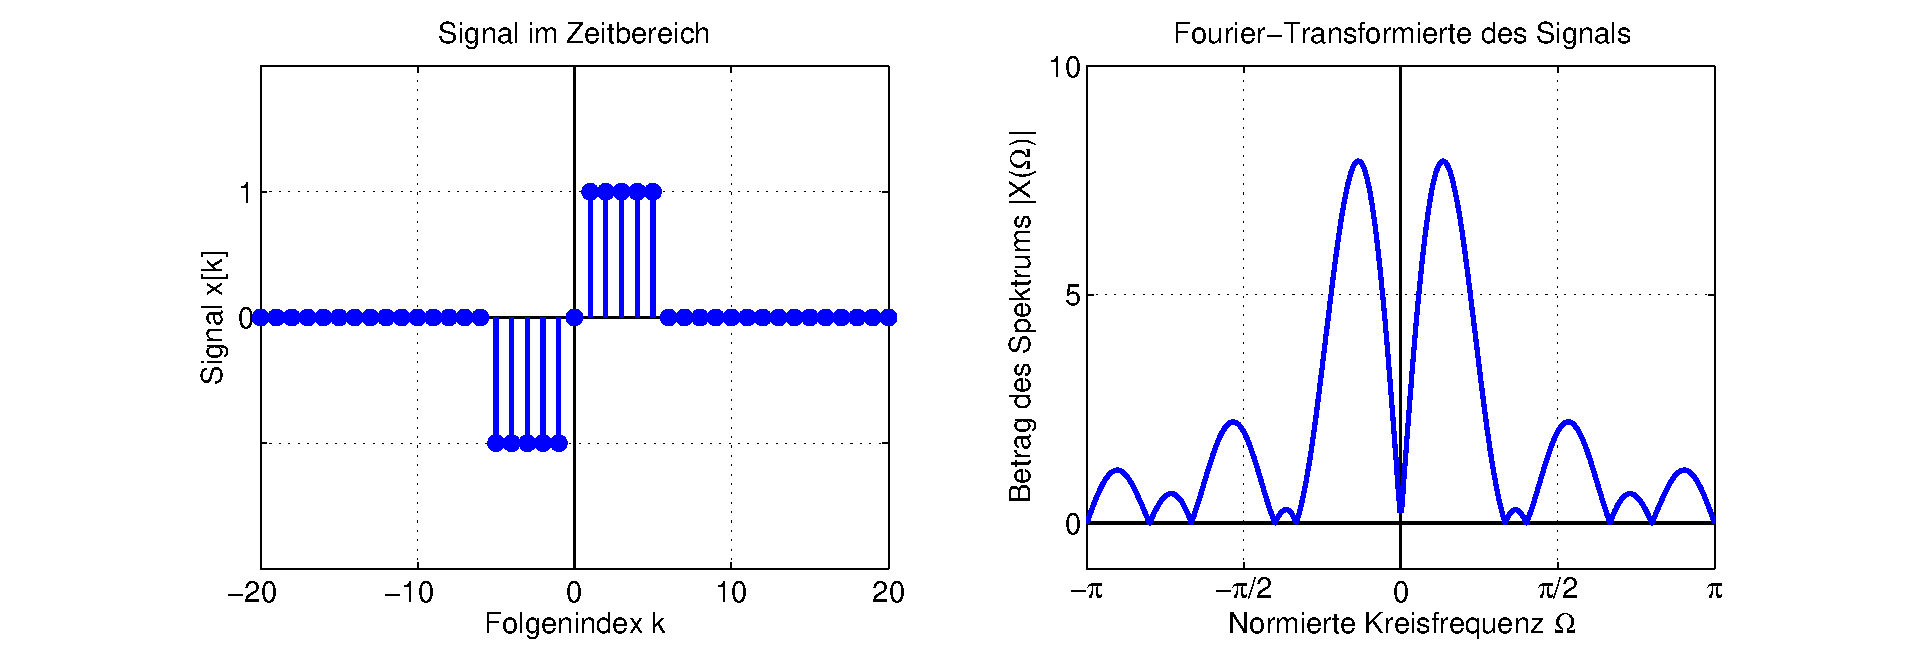
\includegraphics[width=1\textwidth]{Kapitel7/Bilder/image8.eps}}
  \caption{Signalfolge und Betrag des Spektrums f\"{u}r das Beispiel Verschiebung im Zeitbereich kombiniert mit Linearit\"{a}t}
  \label{fig:FourierVerschiebung}
\end{figure}

\clearpage

\subsubsection{Verschiebung im Frequenzbereich}

\noindent Eine Verschiebung kann nicht nur im Zeitbereich, sondern auch im Frequenzbereich erfolgen. In diesem Fall ergibt sich die zugeh\"{o}rige Zeitfunktion aus

\begin{equation}\label{eq:sevenfiftynine}
\begin{split}
X\left(\Omega -\Omega _{0} \right)=\sum _{k=-\infty }^{\infty }x\left[k\right]\cdot e^{-j\cdot k\cdot \left(\Omega -\Omega _{0} \right)} & =\sum _{k=-\infty }^{\infty }x\left[k\right]\cdot e^{-j\cdot k\cdot \Omega } \cdot e^{j\cdot k\cdot \Omega _{0}} \\
&=\sum _{k=-\infty }^{\infty }x\left[k\right]\cdot e^{j\cdot k\cdot \Omega _{0} } \cdot e^{-j\cdot k\cdot \Omega }  =F\left\{x\left[k\right]\cdot e^{j\cdot k\cdot \Omega _{0} } \right\}
\end{split}
\end{equation}

\noindent
\colorbox{lightgray}{%
\arrayrulecolor{white}%
\renewcommand\arraystretch{0.6}%
\begin{tabular}{ wl{16.5cm} }
{\fontfamily{phv}\selectfont{Beispiel: Frequenzverschiebung}}
\end{tabular}%
}\medskip

\noindent Typisches Beispiel f\"{u}r eine Frequenzverschiebung ist eine Modulation. Dabei wird eine Folge x[k] mit einer harmonischen Folge multipliziert.

\begin{equation}\label{eq:sevensixty}
y\left[k\right]=x\left[k\right]\cdot \cos \left(\Omega _{0} \cdot k\right)=x\left[k\right]\cdot \frac{1}{2} \cdot \left(e^{j\cdot \Omega _{0} \cdot k} +e^{-j\cdot \Omega _{0} \cdot k} \right)
\end{equation}

\noindent Durch die Multiplikation verschiebt sich das urspr\"{u}ngliche Spektrum X($\Omega$) um $\Omega_{0}$ nach links und rechts.

\begin{equation}\label{eq:sevensixtyone}
Y\left(\Omega \right)=\frac{1}{2} \cdot \left(X\left(\Omega +\Omega _{0} \right)+X\left(\Omega -\Omega _{0} \right)\right)
\end{equation}

\noindent Das Spektrum wird damit aus dem urspr\"{u}nglichen Spektralbereich in einen Spektralbereich um $\mathrm{\pm}$ $\Omega_{0}$ verschoben. Bild \ref{fig:FourierModulation} stellt die Auswirkung einer Modulation auf den Spektralbereich grafisch dar.

\begin{figure}[H]
  \centerline{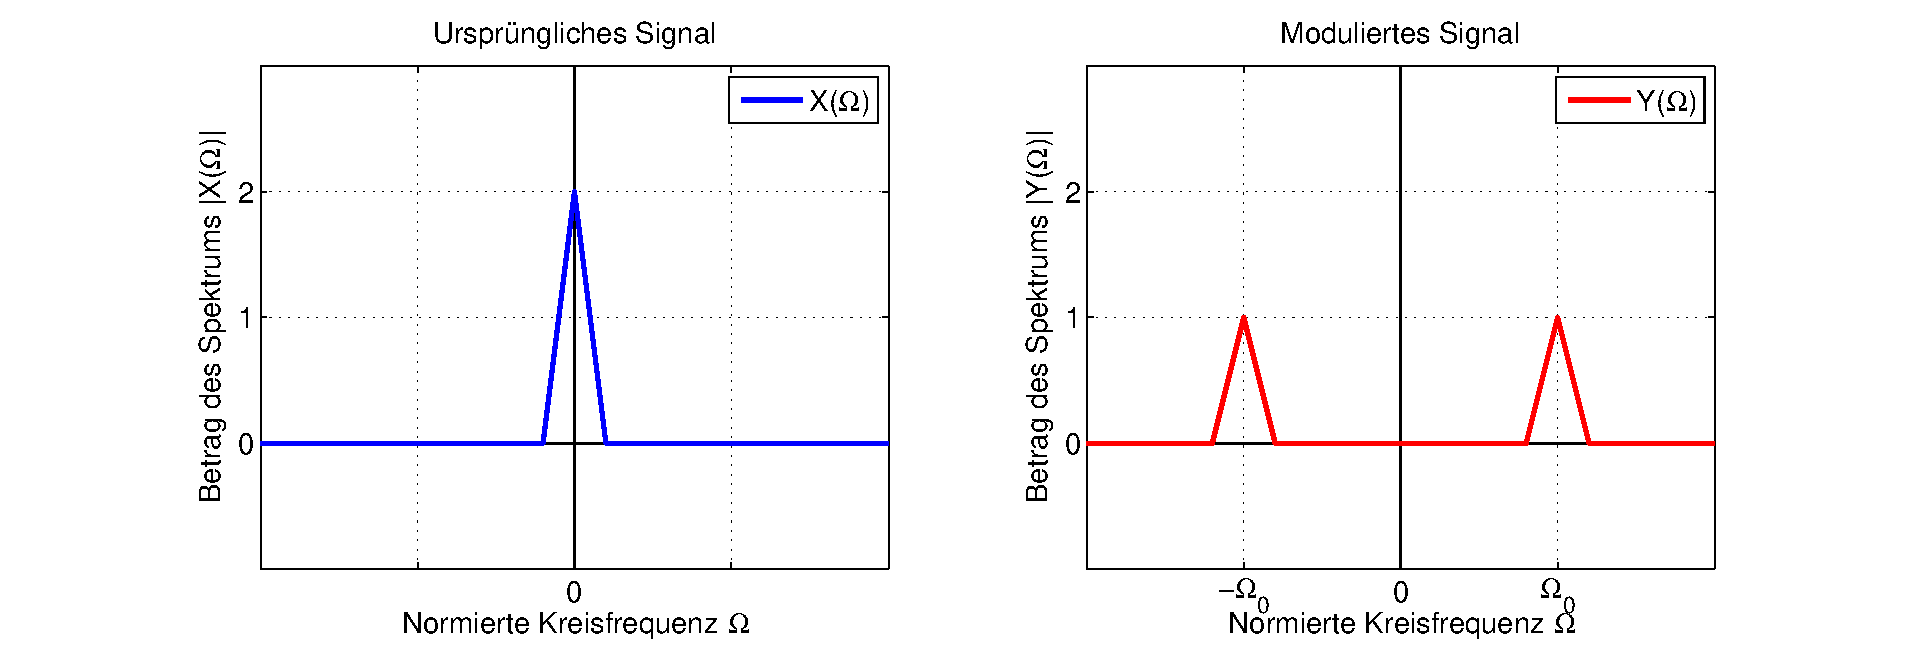
\includegraphics[width=1\textwidth]{Kapitel7/Bilder/image9.eps}}
  \caption{Beispiel f\"{u}r die Verschiebung eines Spektralbereiches durch Modulation}
  \label{fig:FourierModulation}
\end{figure}

\subsubsection{Zeitliche Spiegelung}

\noindent Ist das Spektrum X($\Omega$) einer Signalfolge x[k] bekannt, ergibt sich das Spektrum der Folge x[- k] durch Einsetzen in die Definitionsgleichung zu\bigskip

\begin{equation}\label{eq:sevensixtytwo}
F\left\{x\left[-k\right]\right\}=\sum _{k=-\infty }^{\infty }x\left[-k\right]\cdot e^{-j\cdot \Omega \cdot k}  =\sum _{n=-\infty }^{\infty }x\left[n\right]\cdot e^{j\cdot \Omega \cdot n}  =X\left(-\Omega \right)
\end{equation}

\clearpage

\noindent
\colorbox{lightgray}{%
\arrayrulecolor{white}%
\renewcommand\arraystretch{0.6}%
\begin{tabular}{ wl{16.5cm} }
{\fontfamily{phv}\selectfont{Beispiel: Zeitliche Spiegelung}}
\end{tabular}%
}\medskip

\noindent Als Anwendungen der zeitlichen Spiegelung wird das Spektrum der Folge

\begin{equation}\label{eq:sevensixtythree}
x\left[k\right]=\lambda ^{\left|k\right|}
\end{equation}

f\"{u}r {\textbar}$\lambda${\textbar} $\mathrm{<}$ 1 berechnet werden. Das Spektrum der einseitigen Exponentialfolge wird \"{u}ber die Definitionsgleichung berechnet.

\begin{equation}\label{eq:sevensixtyfour}
F\left\{\lambda ^{k} \cdot \sigma \left[k\right]\right\}=\sum _{k=0}^{\infty }\left(\lambda \cdot e^{-j\cdot \Omega } \right)^{k}  =\frac{1}{1-\lambda \cdot e^{-j\cdot \Omega }}
\end{equation}

\noindent Diese Folge wird achsensymmetrisch erg\"{a}nzt. Das Signal ergibt sich durch die Summe einer kausalen Exponentialfunktion, der gespiegelten Funktion und einer Impulsfolge, die den Wert an der Stelle k = 0 korrigiert.

\begin{equation}\label{eq:sevensixtyfive}
x\left[k\right]=\lambda ^{k} \cdot \sigma \left[k\right]+\lambda ^{-k} \cdot \sigma \left[-k\right]-\delta \left[k\right]
\end{equation}

\noindent Das Spektrum errechnet sich mit der Regel der zeitlichen Spiegelung und der Linearit\"{a}t zu

\begin{equation}\label{eq:sevensixtysix}
X\left(\Omega \right)=\frac{1}{1-\lambda \cdot e^{-j\cdot \Omega } } +\frac{1}{1-\lambda \cdot e^{j\cdot \Omega } } -1
\end{equation}

Die Folge x[k] und der Betrag des Spektrums sind in Bild \ref{fig:FourierZeitinvertierung} dargestellt.

\begin{figure}[H]
  \centerline{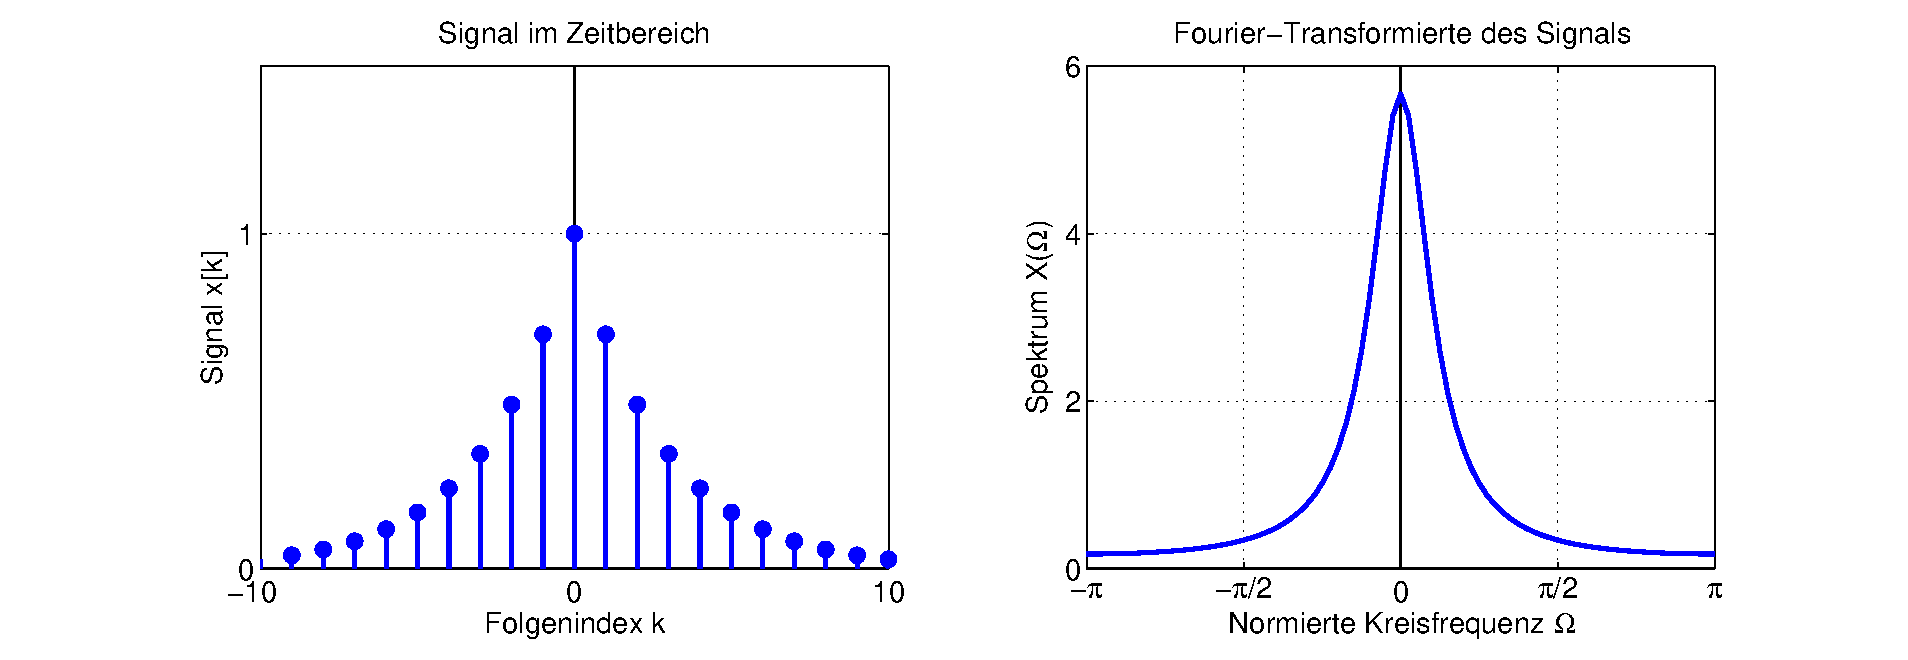
\includegraphics[width=1\textwidth]{Kapitel7/Bilder/image10.eps}}
  \caption{Achsensymmetrische Exponentialfolge und ihr Spektrum für $\lambda$ = 0.7}
  \label{fig:FourierZeitinvertierung}
\end{figure}

\subsubsection{Differenz von Folgen}

\noindent Ist das Spektrum X($\Omega$) einer Signalfolge x[k] bekannt, ergibt sich das Spektrum der Differenz zweier aufeinanderfolgender Folgenwerte x[k] - x[k - 1] durch Anwendung der Verschiebungsregel zu

\begin{equation}\label{eq:sevensixtyseven}
F\left\{x\left[k\right]-x\left[k-1\right]\right\}=X\left(\Omega \right)\cdot \left(1-e^{-j\cdot \Omega } \right)
\end{equation}

\noindent Die Differenzregel ist damit eine Anwendung der Verschiebungsregel. Da die Differenz aber der Differentiation zeitkontinuierlicher Signale entspricht, wird sie als eigene Rechenregel dargestellt.

\subsubsection{Summe von Folgen}

\noindent Ist das Spektrum X($\Omega$) einer Signalfolge x[k] bekannt, ergibt sich das Spektrum der Summe aller Folgenwerte zu

\begin{equation}\label{eq:sevensixtyeight}
F\left\{\sum _{\kappa =-\infty }^{k}x\left[\kappa \right] \right\}=\frac{1}{1-e^{-j\cdot \Omega } } \cdot X\left(\Omega \right)+\pi \cdot X\left(0\right)\cdot \sum _{\nu =-\infty }^{\infty }\delta \left(\Omega +2\cdot \pi \cdot \nu \right)
\end{equation}

\noindent Diese Regel wird ohne Beweis und Beispiel aufgef\"{u}hrt. Der Beweis wird \"{u}ber die Faltungsregel in Kombination mit der Fourier-Transformierten einer Sprungfolge in einer \"{U}bungsaufgabe gef\"{u}hrt. 

\subsubsection{Differentiation im Frequenzbereich}

\noindent Wird das Spektrum X($\Omega$) einer Signalfolge x[k] abgeleitet, wird die Folge im Zeitbereich linear gewichtet. Es ergibt sich die Rechenregel

\begin{equation}\label{eq:sevensixtynine}
F\left\{k\cdot x\left[k\right]\right\}=j\cdot \frac{dX}{d\Omega}
\end{equation}

\noindent Der Beweis ergibt sich aus einer Umformung der Definitionsgleichung.

\begin{equation}\label{eq:sevenseventy}
\frac{dX}{d\Omega } =\frac{d}{d\Omega } \sum _{k=-\infty }^{\infty }x\left[k\right]\cdot e^{-j\cdot \Omega \cdot k}  =\sum _{k=-\infty }^{\infty }-j\cdot k\cdot x\left[k\right]\cdot e^{-j\cdot \Omega \cdot k}  =-j\cdot \sum _{k=-\infty }^{\infty }k\cdot x\left[k\right]\cdot e^{-j\cdot \Omega \cdot k}
\end{equation}

\noindent
\colorbox{lightgray}{%
\arrayrulecolor{white}%
\renewcommand\arraystretch{0.6}%
\begin{tabular}{ wl{16.5cm} }
{\fontfamily{phv}\selectfont{Beispiel: Differentiation im Frequenzbereich}}
\end{tabular}%
}\medskip

\noindent Die Rechenregel zur Differentiation im Frequenzbereich kann dazu verwendet werden, das Spektrum der Folge

\begin{equation}\label{eq:sevenseventyone}
x\left[k\right]=k\cdot \left(\sigma \left[k+K\right]-\sigma \left[k-\left(K+1\right)\right]\right)=k\cdot y\left[k\right]
\end{equation}

\noindent zu berechnen. Mit der Regel f\"{u}r die Differentiation im Frequenzbereich und dem Spektrum der Rechteckfolge y[k] ergibt sich

\begin{equation}\label{eq:sevenseventytwo}
X\left(\Omega \right)=-j\cdot \frac{dY}{d\Omega } =-j\cdot \frac{d}{d\Omega } \frac{\sin \left(K\cdot \Omega \right)}{\sin \left(\frac{\Omega }{2} \right)} =-j\cdot \frac{K\cdot \cos \left(K\cdot \Omega \right)\cdot \sin \left(\frac{\Omega }{2} \right)-\frac{1}{2} \cdot \cos \left(\frac{\Omega }{2} \right)\cdot \sin \left(K\cdot \Omega \right)}{\sin ^{2} \left(\frac{\Omega }{2} \right)}
\end{equation}

\subsubsection{Faltung im Zeitbereich}

\noindent Das Ausgangssignal zeitdiskreter LTI-System errechnet sich \"{u}ber die Faltungssumme.

\begin{equation}\label{eq:sevenseventythree}
y\left[k\right]=g\left[k\right]*u\left[k\right]=\sum _{\kappa =-\infty }^{\infty }g\left[\kappa \right]\cdot u\left[k-\kappa \right] =\sum _{\kappa =-\infty }^{\infty }g\left[k-\kappa \right] \cdot u\left[\kappa \right]
\end{equation}

\noindent Sind die Spektren G($\Omega$) der Signalfolge g[k] und U($\Omega$) der Signalfolge u[k] bekannt, errechnet sich das Spektrum des Ausgangssignals \"{u}ber das Produkt der beiden Spektren

\begin{equation}\label{eq:sevenseventyfour}
Y\left(\Omega \right)=G\left(\Omega \right)\cdot U\left(\Omega \right)
\end{equation}

\noindent Der Beweis kann wie bei der z-Transformation durch Einsetzen in die Definitionsgleichung gef\"{u}hrt werden. 

\begin{equation}\label{eq:sevenseventyfive}
F\left\{g\left[k\right]*u\left[k\right]\right\}=F\left\{\sum _{\kappa =-\infty }^{\infty }g\left[\kappa \right]\cdot u\left[k-\kappa \right] \right\}=\sum _{k=-\infty }^{\infty }\sum _{\kappa =-\infty }^{\infty }g\left[\kappa \right]\cdot u\left[k-\kappa \right]  \cdot e^{-j\cdot \Omega \cdot k}
\end{equation}

\noindent Vertauschen der Summationsreihenfolge und Substitution ergibt

\begin{equation}\label{eq:sevenseventysix}
\begin{split}
F\left\{g\left[k\right]*u\left[k\right]\right\} &=\sum _{k=-\infty }^{\infty }\sum _{\kappa =-\infty }^{\infty }g\left[\kappa \right]\cdot u\left[k-\kappa \right]  \cdot e^{-j\cdot \Omega \cdot k} =\sum _{\kappa =-\infty }^{\infty}\sum _{k=-\infty }^{\infty }g\left[\kappa \right]\cdot u\left[k-\kappa \right]  \cdot e^{-j\cdot \Omega \cdot k}\\
&=\sum _{\kappa =-\infty }^{\infty}g\left[\kappa \right]\cdot \sum _{k=-\infty }^{\infty}u\left[k-\kappa \right]  \cdot e^{-j\cdot \Omega \cdot k}\cdot e^{j\cdot \Omega \cdot \kappa}\cdot e^{-j\cdot \Omega \cdot \kappa}\\
&=\sum _{n =-\infty }^{\infty}g\left[\kappa \right]\cdot e^{-j\cdot \Omega \cdot \kappa}\cdot \sum _{k=-\infty }^{\infty}u\left[k-\kappa \right]  \cdot e^{-j\cdot \Omega \cdot(k- \kappa)}=\sum _{n =-\infty }^{\infty}g\left[n \right]\cdot e^{-j\cdot \Omega \cdot n}\cdot \sum _{m=-\infty }^{\infty}u\left[m \right]  \cdot e^{-j\cdot \Omega \cdot m}\\
&=G(\Omega)\cdot U(\Omega)
\end{split}
\end{equation}

\noindent Die Faltungsregel ist eine wesentliche Rechenregel der Fourier-Transformation f\"{u}r Signalfolgen, da sich das Ausgangssignal eines linearen zeitinvarianten Systems aus der Faltung von Eingangsfolge und Impulsantwort ergibt. Die Faltungsregel wird im Kapitel 1 detailliert aufgegriffen.

\subsubsection{Multiplikation im Zeitbereich}

\noindent Neben der Faltung ist bei der digitalen Signalverarbeitung die Multiplikation im Zeitbereich eine wichtige Operation. Sie wird verwendet, um den Ausschnitt eines Signals zu beschreiben, indem das Signal x[k] mit einer sogenannten Fensterfunktion w[k] multipliziert wird. Die Rechenregel zur Multiplikation im Zeitbereich erm\"{o}glicht die Berechnung des Spektrums von dem Signalausschnitt.

\noindent Sind die Spektren X($\Omega$) einer Signalfolge x[k] und W($\Omega$) einer Signalfolge w[k] bekannt, errechnet sich das Spektrum des Signals, das aus dem Produkt der beiden Signale

\begin{equation}\label{eq:sevenseventyseven}
y\left[k\right]\; =\; x\left[k\right]\cdot w\left[k\right]
\end{equation}

\noindent entsteht, durch Einsetzen der Signale in die Definitionsgleichung

\begin{equation}\label{eq:sevenseventyeight}
Y\left(\Omega \right)=\sum _{k=-\infty }^{\infty }x\left[k\right]\cdot w\left[k\right] \cdot e^{-j\cdot \Omega \cdot k}
\end{equation}

\noindent Die Substitution der Folge w[k] durch ihre inverse Fourier-Transformierte 

\begin{equation}\label{eq:sevenseventynine}
Y\left(\Omega \right)=\sum _{k=-\infty}^{\infty}x\left[k\right]\cdot \frac{1}{2\cdot \pi} \cdot \int\limits _{-\pi}^{\pi}W\left(\Theta \right)\cdot e^{j\cdot k\cdot \Theta} d\Theta \cdot e^{-j\cdot \Omega \cdot k}
\end{equation}

\noindent und Tauschen der Reihenfolge von Integration und Summation 

\begin{equation}\label{eq:sevenseighty}
Y\left(\Omega \right)=\sum _{k=-\infty }^{\infty }x\left[k\right]\cdot \frac{1}{2\cdot \pi}\cdot \int\limits _{-\pi}^{\pi}W\left(\Theta \right)\cdot e^{j\cdot k\cdot \Theta } d\Theta \cdot e^{-j\cdot \Omega \cdot k} =\frac{1}{2\cdot \pi } \cdot \int\limits _{-\pi}^{\pi}W\left(\Theta \right)\cdot \sum _{k=-\infty}^{\infty}x\left[k\right]\cdot e^{j\cdot \left(\Theta -\Omega \right)\cdot k} d\Theta 
\end{equation}

\noindent f\"{u}hrt unter Anwendung der Verschiebungsregel im Frequenzbereich zu

\begin{equation}\label{eq:sevenseightyone}
\begin{split}
Y\left(\Omega \right) &=\frac{1}{2\cdot \pi} \cdot \int\limits _{-\pi}^{\pi}W\left(\Theta \right)\cdot \sum _{k=-\infty }^{\infty }x\left[k\right]\cdot e^{j\cdot \left(\Theta -\Omega \right)\cdot k}d\Theta  =\frac{1}{2\cdot \pi } \cdot \int\limits _{-\pi}^{\pi}W\left(\Theta \right)\cdot X\left(\Omega -\Theta \right)d\Theta \\
&=\frac{1}{2\cdot \pi} \cdot X(\Omega)*W(\Omega)
\end{split}
\end{equation}

\noindent Die Multiplikation zweier Folgen im Zeitbereich f\"{u}hrt demnach zu einer Faltung der entsprechenden Spektren im Frequenzbereich.\bigskip

\noindent
\colorbox{lightgray}{%
\arrayrulecolor{white}%
\renewcommand\arraystretch{0.6}%
\begin{tabular}{ wl{16.5cm} }
{\fontfamily{phv}\selectfont{Beispiel: Fensterung als Multiplikation im Zeitbereich}}
\end{tabular}%
}\medskip

\noindent Als Beispiel wird eine Kosinusfolge betrachtet, von der ein Ausschnitt \"{u}ber zwei Periodendauern vorliegt. Der Signalausschnitt ist in Bild 7.11 dargestellt und kann mathematisch beschrieben werden als 

\begin{equation}\label{eq:sevenseightytwo}
\begin{split}
y\left[k\right] &=w\left[k\right]\cdot x\left[k\right]=\left(\sigma \left[k+10\right]-\sigma \left[k-11\right]\right)\cdot \cos \left(\frac{2\cdot \pi }{10} \cdot k\right) \\ 
&=\left(\sigma \left[k+10\right]-\sigma \left[k-11\right]\right)\cdot \cos \left(\frac{\pi }{5} \cdot k\right)
\end{split}
\end{equation}

\noindent Das Spektrum der Folge w[k] ergibt sich aus der berechneten Rechteckfolge und der Verschiebungsregel zu

\begin{equation}\label{eq:sevenseightythree}
W\left(\Omega \right)=\frac{\sin \left(\frac{21\cdot \Omega }{2} \right)}{\sin \left(\frac{\Omega }{2} \right)}
\end{equation}

\noindent Das Spektrum der Kosinusfolge x[k] wird berechnet zu

\begin{equation}\label{eq:sevenseightyfour}
X\left(\Omega \right)=\pi \cdot \left(\delta \left(\Omega +\frac{\pi }{5} \right)+\delta \left(\Omega -\frac{\pi }{5} \right)\right)
\end{equation}

\noindent Die Multiplikation im Zeitbereich f\"{u}hrt zu Faltung im Frequenzbereich. Die Faltung der beiden Spektren f\"{u}hrt zu einer Verschiebung von W($\Omega$) an die Stellen der Impulse. Damit ergibt sich f\"{u}r das Spektrum Y($\Omega$)

\begin{equation}\label{eq:sevenseightyfive}
\begin{split}
Y\left(\Omega \right) &=\frac{1}{2\cdot \pi } \cdot \pi \cdot \left(\frac{\sin \left(\frac{21\cdot \left(\Omega +\frac{\pi }{5} \right)}{2} \right)}{\sin \left(\frac{\left(\Omega +\frac{\pi }{5} \right)}{2} \right)} +\frac{\sin \left(\frac{21\cdot \left(\Omega -\frac{\pi }{5} \right)}{2} \right)}{\sin \left(\frac{\left(\Omega -\frac{\pi }{5} \right)}{2} \right)} \right) \\ 
& =\frac{1}{2} \cdot \left(\frac{\sin \left(21\cdot \left(\frac{\Omega }{2} +\frac{\pi }{10} \right)\right)}{\sin \left(\frac{\Omega }{2} +\frac{\pi }{10} \right)} +\frac{\sin \left(21\cdot \left(\frac{\Omega }{2} -\frac{\pi }{10} \right)\right)}{\sin \left(\frac{\Omega }{2} -\frac{\pi }{10} \right)} \right)
\end{split}
\end{equation}

\noindent Signal und Betrag des Spektrums sind in Bild \ref{fig:FourierFensterung} dargestellt.

\begin{figure}[H]
  \centerline{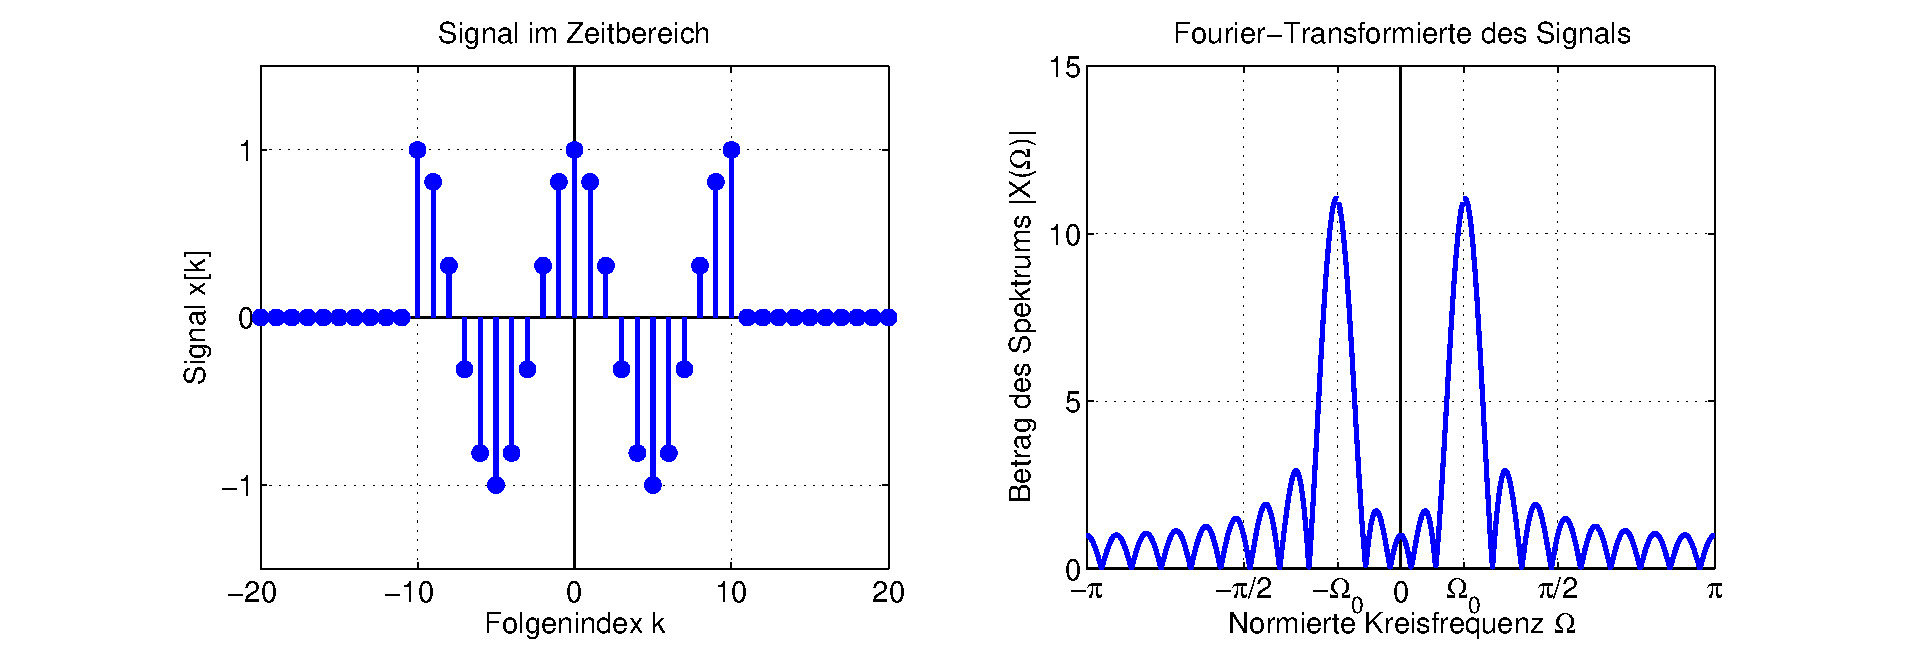
\includegraphics[width=1\textwidth]{Kapitel7/Bilder/image11.eps}}
  \caption{Ausschnitt einer Kosinusfolge und das entsprechende Spektrum}
  \label{fig:FourierFensterung}
\end{figure}

\noindent Durch die Multiplikation der Folge mit einer Rechteckfolge wird das Signal ausgeschnitten. Im Frequenzbereich falten sich die Spektren der beiden Signale, wobei das Spektrum der Kosinusfunktion aus zwei Impulsen an den Stellen $\mathrm{\pm}$ $\Omega_{0}$ besteht. Durch die Faltung wird das Spektrum der Rechteckfolge an die Stellen $\mathrm{\pm}$ $\Omega_{0}$ verschoben. Der Effekt, der bei der Fensterung von Signalen entsteht, wird bei der Sch\"{a}tzung von Spektren in Kapitel 1 weiter vertieft. Zus\"{a}tzlich wird das Spektrum wegen der Abtastung periodisch in 2$\cdot\piup$ wiederholt.

\subsubsection{Parsevalsche Gleichung}

\noindent Die Parsevalsche Gleichung dr\"{u}ckt aus, dass die Summe \"{u}ber dem Quadrat einer Folge gleich dem Integral \"{u}ber dem Quadrat ihrer Transformierten ist. Wie bei zeitkontinuierlichen Signalen wird es dazu verwendet, die Energie eines Signals im Zeitbereich oder im Frequenzbereich zu berechnen.

\begin{equation}\label{eq:sevenseightysix}
E=\sum _{k=-\infty }^{\infty }x\left[k\right]\cdot x^{*} \left[k\right] =\frac{1}{2\cdot \pi } \cdot \int _{-\pi }^{\pi }X\left(\Omega \right)\cdot X^{*} \left(\Omega \right)d\Omega
\end{equation}

\noindent Der Beweis dieser Rechenregel ergibt sich aus der Faltungsregel. Der linke Teil der Gleichung entspricht der Faltungssumme von x[k] und x*[- k] an der Stelle k = 0.

\begin{equation}\label{eq:sevenseightyseven}
\left. x\left[k\right]*x^{*} \left[-k\right]\right|_{k=0} =\left. \sum _{\kappa =-\infty }^{\infty }x\left[\kappa \right]\cdot x^{*} \left[-\left(k-\kappa \right)\right] \right|_{k=0} =\left. \sum _{\kappa =-\infty }^{\infty }x\left[\kappa \right]\cdot x^{*} \left[-k+\kappa \right] \right|_{k=0} =\sum _{\kappa =-\infty }^{\infty }x\left[\kappa \right]\cdot x^{*} \left[\kappa \right]
\end{equation}

\noindent Der Faltung im Zeitbereich entspricht die Multiplikation im Frequenzbereich. Mit den Spektren

\begin{equation}\label{eq:sevenseightyeight}
x\left[k\right]\circ -\bullet X\left(\Omega \right)
\end{equation}

\noindent und

\begin{equation}\label{eq:sevenseightynine}
x^{*} \left[-k\right]\circ -\bullet X^{*} \left(\Omega \right)
\end{equation}

\noindent sowie der Definitionsgleichung f\"{u}r die inverse Fourier-Transformierte an der Stelle k = 0 ergibt sich

\begin{equation}\label{eq:sevenninety}
\sum _{\kappa =-\infty}^{\infty}x\left[\kappa \right]\cdot x^{*} \left[\kappa \right] =\left. \frac{1}{2\cdot \pi} \cdot \int\limits _{-\pi}^{\pi}X\left(\Omega \right)\cdot X^{*} \left(\Omega \right)\cdot e^{j\cdot k\cdot \Omega}d\Omega \right|_{k=0} =\frac{1}{2\cdot \pi} \cdot \int\limits _{-\pi}^{\pi}X\left(\Omega \right)\cdot X^{*} \left(\Omega \right)d\Omega
\end{equation}

\noindent Der Ausdruck X($\Omega$)$\cdot$X*($\Omega$) entspricht dem Betragsquadrat {\textbar}X($\Omega$){\textbar}${}^{2}$ und wird als Energiedichtespektrum bezeichnet. Es ist insbesondere bei der Berechnung stochastischer Prozesse von Bedeutung und wird in Teil C dieser Buchreihe wieder aufgegriffen.

\subsubsection{Zusammenfassung der Rechenregeln zur Fourier-Transformation von Signalfolgen}

\noindent Zur besseren \"{U}bersicht stellt Tabelle \ref{tab:sevenfour} die wesentlichen Eigenschaften der Fourier-Transformation von Signalfolgen noch einmal zusammen.
\clearpage
\begin{table}[H]
\setlength{\arrayrulewidth}{.1em}
\caption{Rechenregeln der Fourier-Transformation von Signalfolgen}
\setlength{\fboxsep}{0pt}%
\colorbox{lightgray}{%
\arrayrulecolor{white}%
\begin{tabular}{| c | c | c |}
\hline
\parbox[c][0.3in][c]{1.6in}{\smallskip\centering\textbf{\fontfamily{phv}\selectfont{Regel}}} & \parbox[c][0.3in][c]{1.8in}{\smallskip\centering\textbf{\fontfamily{phv}\selectfont{Funktion x(t)}}} &
\parbox[c][0.3in][c]{2.9in}{\smallskip\centering\textbf{\fontfamily{phv}\selectfont{Laplace-Transformierte X(s)}}}\\ \hline


\parbox[c][0.5in][c]{1.6in}{\centering{\fontfamily{phv}\selectfont{Linearität}}} & 
\parbox[c][0.5in][c]{1.8in}{\centering{$\nu _{1} \cdot x_{1} \left(k\right)+\nu _{2} \cdot x_{2} \left(k\right)$}} &
\parbox[c][0.5in][c]{2.9in}{\centering{$\nu _{1} \cdot X_{1} \left(\Omega\right)+\nu _{2} \cdot X_{2} \left(\Omega\right)$}}\\
\hline

\parbox[c][0.5in][c]{1.6in}{\centering{\fontfamily{phv}\selectfont{Zeitverschiebung}}} & 
\parbox[c][0.5in][c]{1.8in}{\centering{$x\left[k-k_{0} \right]$}} &
\parbox[c][0.5in][c]{2.9in}{\centering{$e^{-j\cdot \Omega \cdot k_{0}}\cdot X\left(\Omega \right)$}}\\
\hline

\parbox[c][0.5in][c]{1.6in}{\centering{\fontfamily{phv}\selectfont{Frequenzverschiebung}}} & 
\parbox[c][0.5in][c]{1.8in}{\centering{$x\left[k\right]\cdot e^{j\cdot k\cdot \Omega _{0}}$}} &
\parbox[c][0.5in][c]{2.9in}{\centering{$X\left(\Omega -\Omega _{0} \right)$}}\\
\hline

\parbox[c][0.5in][c]{1.6in}{\centering{\fontfamily{phv}\selectfont{Zeitliche Spiegelung}}} & 
\parbox[c][0.5in][c]{1.8in}{\centering{$x\left[-k\right]$}} &
\parbox[c][0.5in][c]{2.9in}{\centering{$X\left(-\Omega \right)$}}\\
\hline

\parbox[c][0.5in][c]{1.6in}{\centering{\fontfamily{phv}\selectfont{Differenz}}} & 
\parbox[c][0.5in][c]{1.8in}{\centering{$x\left[k\right]-x\left[k-1\right]$}} &
\parbox[c][0.5in][c]{2.9in}{\centering{$X\left(\Omega \right)\cdot \left(1-e^{-j\cdot \Omega } \right)$}}\\
\hline

\parbox[c][0.7in][c]{1.6in}{\centering{\fontfamily{phv}\selectfont{Summation}}} & 
\parbox[c][0.7in][c]{1.8in}{\centering{$\sum _{\kappa =-\infty }^{k}x\left[\kappa \right]$}} &
\parbox[c][0.7in][c]{2.9in}{\centering{$\frac{1}{1-e^{-j\cdot \Omega } } \cdot X\left(\Omega \right)+\pi \cdot X\left(0\right)\cdot \sum _{\nu =-\infty }^{\infty }\delta \left(\Omega +2\cdot \pi \cdot \nu \right) $}}\\
\hline

\parbox[c][0.5in][c]{1.6in}{\centering{\fontfamily{phv}\selectfont{lineare Gewichtung}}} & 
\parbox[c][0.5in][c]{1.8in}{\centering{$k\cdot x\left[k\right]$}} &
\parbox[c][0.5in][c]{2.9in}{\centering{$j\cdot \frac{dX}{d\Omega }$}}\\
\hline

\parbox[c][0.5in][c]{1.6in}{\centering{\fontfamily{phv}\selectfont{Faltung}}} & 
\parbox[c][0.5in][c]{1.8in}{\centering{$g\left[k\right]*u\left[k\right]$}} &
\parbox[c][0.5in][c]{2.9in}{\centering{$G\left(\Omega \right)\cdot U\left(\Omega \right)$}}\\
\hline

\parbox[c][0.5in][c]{1.6in}{\centering{\fontfamily{phv}\selectfont{Multiplikation}}} & 
\parbox[c][0.5in][c]{1.8in}{\centering{$x\left[k\right]\cdot w\left[k\right]$}} &
\parbox[c][0.5in][c]{2.9in}{\centering{$\frac{1}{2\cdot \pi } \cdot X\left(\Omega \right)*W\left(\Omega \right)$}}\\
\hline

\parbox[c][0.7in][c]{1.6in}{\centering{\fontfamily{phv}\selectfont{Parsevalsche Gleichung}}} & 
\parbox[c][0.7in][c]{1.8in}{\centering{$E=\sum _{k=-\infty }^{\infty }x\left[k\right]\cdot x^{*} \left[k\right]$}} &
\parbox[c][0.7in][c]{2.9in}{\centering{$E=\frac{1}{2\cdot \pi} \cdot \int\limits_{-\pi}^{\pi}X\left(\Omega \right)\cdot X^{*} \left(\Omega \right)d\Omega $}}\\
\hline

\end{tabular}%
}
\label{tab:sevenfour}
\end{table}

\noindent Mit Hilfe der zusammengestellten Rechenregeln lassen sich weitere Korrespondenzen bestimmen. 

\clearpage

\noindent
\colorbox{lightgray}{%
\arrayrulecolor{white}%
\renewcommand\arraystretch{0.6}%
\begin{tabular}{ wl{16.5cm} }
{\fontfamily{phv}\selectfont{Beispiel: Fourier-Transformierte der Sprungfolge}}
\end{tabular}%
}\medskip

\noindent Die Rechenregeln der zeitdiskreten Fourier-Transformation werden angewendet, um die Korrespondenz der Sprungfolge zu bestimmen. Die Sprungfolge kann in zwei Anteile zerlegt werden, in die konstante Folge 

\begin{equation}\label{eq:sevenninetyone}
x_{1} \left[k\right]=0.5
\end{equation}

\noindent und die Folge

\begin{equation}\label{eq:sevenninetytwo}
x_{2} \left[k\right]=\left\{\begin{array}{l} {-0.5\quad \text{ für k }<0} \\ {+0.5\quad \text{ für k }\ge 0} \end{array}\right. 
\end{equation}

\begin{figure}[H]
  \centerline{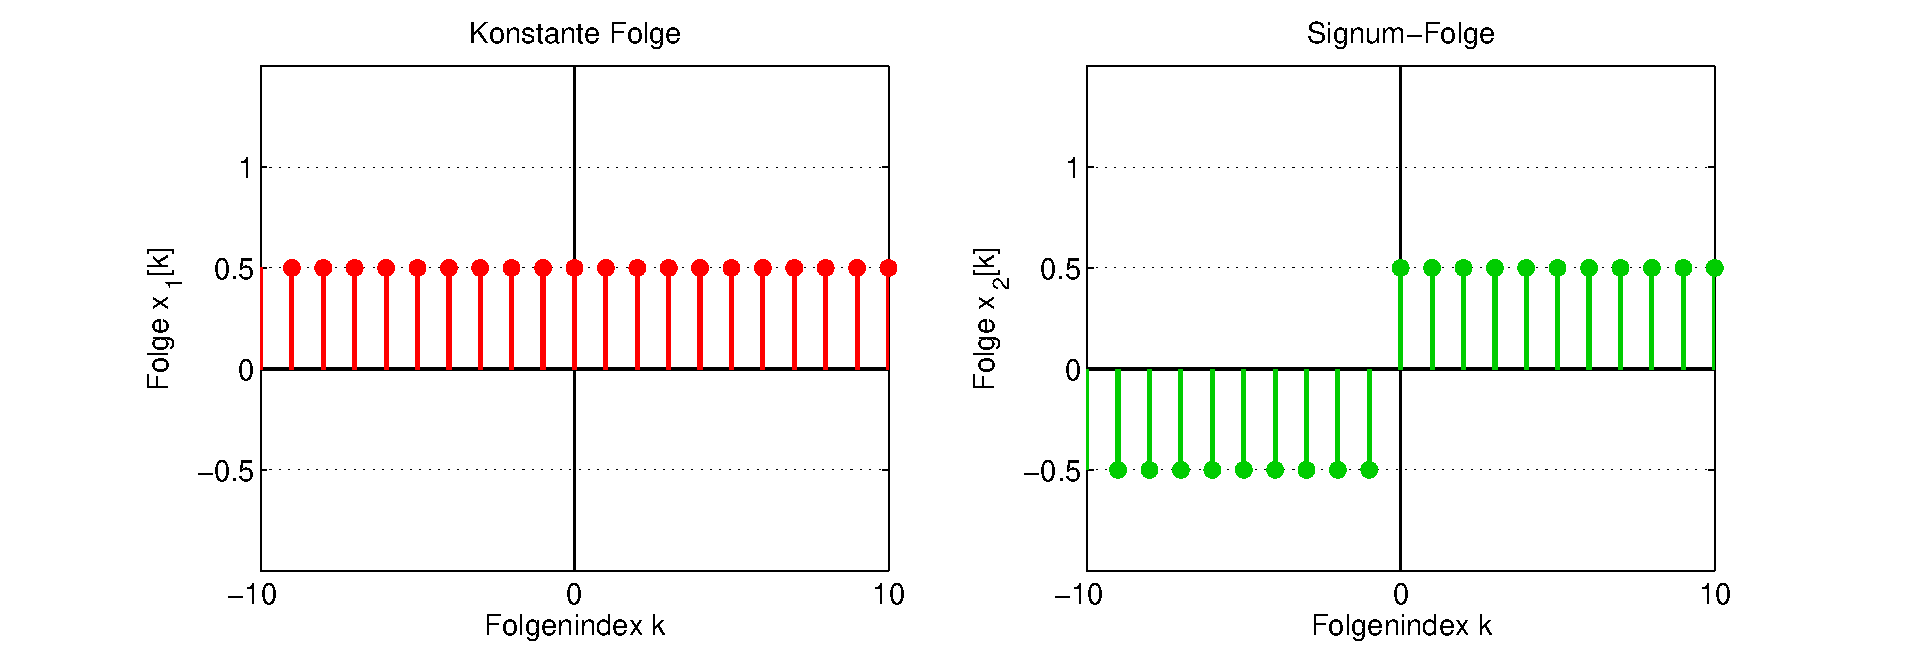
\includegraphics[width=1\textwidth]{Kapitel7/Bilder/image12.eps}}
  \caption{Zerlegung der Sprungfolge in eine konstante Folge und eine Signum-Folge}
  \label{fig:FourierSprungfolge}
\end{figure}

\noindent Die Summe der beiden Folgen ergibt die Sprungfolge. F\"{u}r den Teil x${}_{1}$[k] kann die Fourier-Transformierte mit der Korrespondenz der Einsfolge und der Linearit\"{a}t angegeben werden zu

\begin{equation}\label{eq:sevenninetythree}
X_{1} \left(\Omega \right)=\pi \cdot \sum _{\nu =-\infty }^{\infty }\delta \left(\Omega -2\cdot \pi \cdot \nu \right)
\end{equation}

\noindent Zur Ermittlung der Fourier-Transformierten des zweiten Teils x${}_{2}$[k] wird die Impulsfolge verwendet. Sie kann dargestellt werden als

\begin{equation}\label{eq:sevenninetytfour}
\delta \left[k\right]=x_{2} \left[k\right]-x_{2} \left[k-1\right]
\end{equation}

\noindent Die Fourier-Transformierte der Impulsfolge ist 1 und eine Verschiebung der Funktion um k${}_{0}$ = 1 f\"{u}hrt zur Multiplikation der Fourier-Transformierten mit e${}^{-j}$. Damit ergibt sich f\"{u}r die Fourier-Transformierte 

\begin{equation}\label{eq:sevenninetytfive}
1=\left(1-e^{-j\cdot \Omega } \right)\cdot \sum _{k=-\infty }^{\infty }x_{2} \left[k\right]\cdot e^{-j\cdot \Omega \cdot k}  =\left(1-e^{-j\cdot \Omega } \right)\cdot X_{2} \left(e^{j\cdot \Omega } \right)
\end{equation}

\noindent und durch Aufl\"{o}sen

\begin{equation}\label{eq:sevenninetytsix}
X_{2} \left(\Omega \right)=\frac{1}{1-e^{-j\cdot \Omega}}
\end{equation}

\noindent Durch Superposition von Gleichung \eqref{eq:sevenninetythree} und Gleichung \eqref{eq:sevenninetytsix} ergibt sich die Fourier-Transformierte des diskreten Einheitssprungs zu 

\begin{equation}\label{eq:sevenninetytseven}
F\left(\sigma \left[k\right]\right)=\frac{1}{1-e^{-j\cdot \Omega } } +\pi \cdot \sum _{\nu =-\infty }^{\infty }\delta \left(\Omega -2\cdot \pi \cdot \nu \right)
\end{equation}

\noindent Bild \ref{fig:FourierSprungfolge1} stellt den diskreten Einheitssprung und den Betrag seiner Fourier-Transformierten gegen\"{u}ber.

\begin{figure}[H]
  \centerline{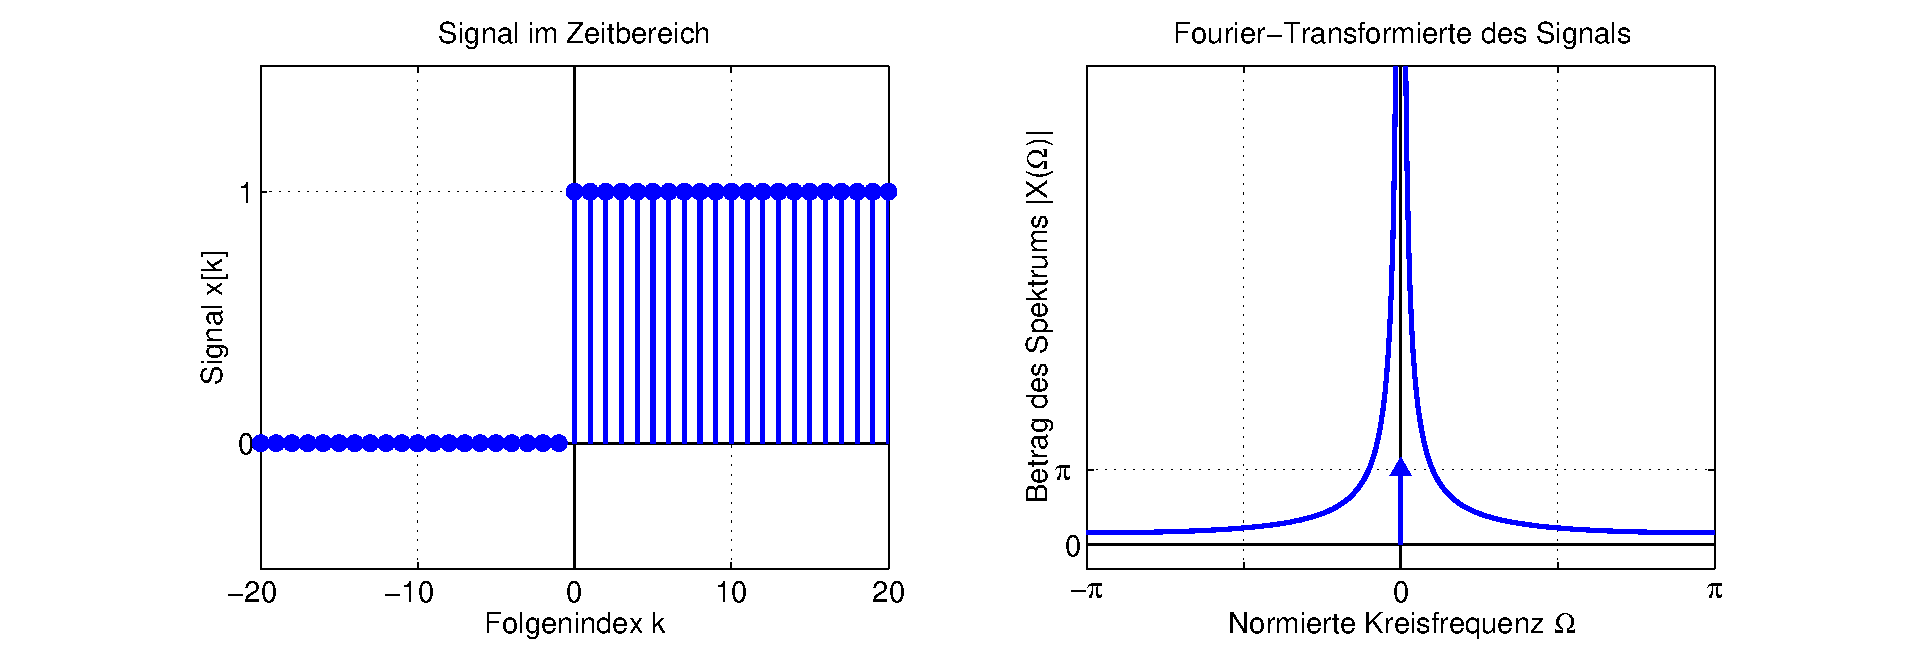
\includegraphics[width=1\textwidth]{Kapitel7/Bilder/image13.eps}}
  \caption{Diskreter Einheitssprung und der Betrag seines Spektrums}
  \label{fig:FourierSprungfolge1}
\end{figure}

\clearpage

\subsubsection{Korrespondenzen der Fourier-Transformation von Signalfolgen}

\noindent Tabelle \ref{tab:sevenfive} stellt wichtige Korrespondenzen der Fourier-Transformation von Signalfolgen zusammen.

\begin{table}[H]
\setlength{\arrayrulewidth}{.1em}
\caption{Korrespondenzen der Laplace-Transformation (2/2)}
\setlength{\fboxsep}{0pt}%
\colorbox{lightgray}{%
\arrayrulecolor{white}%
\begin{tabular}{| c | c | c |}
\hline
\parbox[c][0.3in][c]{0.3in}{\smallskip\centering\textbf{\fontfamily{phv}\selectfont{Nr}}} &
\parbox[c][0.3in][c]{2.7in}{\smallskip\centering\textbf{\fontfamily{phv}\selectfont{Folge x[k]}}} & 
\parbox[c][0.3in][c]{3.3in}{\smallskip\centering\textbf{\fontfamily{phv}\selectfont{Fourier-Transformierte X($\Omega$)}}}\\ \hline

\parbox[c][0.5in][c]{0.3in}{\centering{1}} &
\parbox[c][0.5in][c]{2.7in}{\centering{$\delta \left[k\right]$}} & 
\parbox[c][0.5in][c]{3.3in}{\centering{1}}\\ \hline

\parbox[c][0.5in][c]{0.3in}{\centering{2}} &
\parbox[c][0.5in][c]{2.7in}{\centering{1}} & 
\parbox[c][0.5in][c]{3.3in}{\centering{$2\cdot \pi \cdot \sum _{\nu =-\infty }^{\infty }\delta \left(\Omega +2\cdot \pi \cdot \nu \right)$}}\\ \hline

\parbox[c][0.5in][c]{0.3in}{\centering{3}} &
\parbox[c][0.5in][c]{2.7in}{\centering{$\delta \left[k-k_{0} \right]$}} & 
\parbox[c][0.5in][c]{3.3in}{\centering{$e^{-j\cdot \Omega \cdot k_{0} } $}}\\ \hline

\parbox[c][0.5in][c]{0.3in}{\centering{4}} &
\parbox[c][0.5in][c]{2.7in}{\centering{$\lambda ^{k} \cdot \sigma \left[k\right]$}} & 
\parbox[c][0.5in][c]{3.3in}{\centering{$\frac{1}{1-\lambda \cdot e^{-j\cdot \Omega}}\quad \;\;$ für $\left|\lambda \right|<1$}}\\ \hline

\parbox[c][0.5in][c]{0.3in}{\centering{5}} &
\parbox[c][0.5in][c]{2.7in}{\centering{$(k+1)\cdot \lambda ^{k} \cdot \sigma \left[k\right]$}} & 
\parbox[c][0.5in][c]{3.3in}{\centering{$\frac{1}{\left(1-\lambda \cdot e^{-j\cdot \Omega } \right)^{2}}\;$ für $\left|\lambda \right|<1$}}\\ \hline

\parbox[c][0.5in][c]{0.3in}{\centering{6}} &
\parbox[c][0.5in][c]{2.7in}{\centering{$\sigma \left[k\right]$}} & 
\parbox[c][0.5in][c]{3.3in}{\centering{$\frac{1}{1-e^{-j\cdot \Omega } } +\pi \cdot \sum _{\nu =-\infty }^{\infty }\delta \left(\Omega +2\cdot \pi \cdot \nu \right) $}}\\ \hline

\parbox[c][0.5in][c]{0.3in}{\centering{7}} &
\parbox[c][0.5in][c]{2.7in}{\centering{$e^{j\cdot \Omega \cdot k_{0}}$}} & 
\parbox[c][0.5in][c]{3.3in}{\centering{$2\cdot \pi \cdot \sum _{\nu =-\infty }^{\infty }\delta \left(\Omega -\Omega _{0} +2\cdot \pi \cdot \nu \right)$}}\\ \hline

\parbox[c][0.7in][c]{0.3in}{\centering{8}} &
\parbox[c][0.7in][c]{2.7in}{\centering{$x\left[k\right]=\sigma \left[k\right]-\sigma \left[k-k_{0} \right]$}} & 
\parbox[c][0.7in][c]{3.3in}{\centering{$e^{-j\cdot \frac{\Omega \cdot \left(k_{0} -1\right)}{2} } \cdot \frac{\sin \left(\frac{k_{0} \cdot \Omega }{2} \right)}{\sin \left(\frac{\Omega }{2} \right)} $}}\\ \hline

\parbox[c][0.7in][c]{0.3in}{\centering{9}} &
\parbox[c][0.7in][c]{2.7in}{\centering{$\sin \left[\Omega _{0} \cdot k\right]$}} & 
\parbox[c][0.7in][c]{3.3in}{\centering{$j\cdot \pi \cdot \sum _{n=-\infty }^{\infty }\delta \left(\Omega +\Omega _{0} +2\cdot \pi \cdot n\right)-\delta \left(\Omega -\Omega _{0} +2\cdot \pi \cdot n\right) $}}\\ \hline

\parbox[c][0.5in][c]{0.3in}{\centering{10}} &
\parbox[c][0.5in][c]{2.7in}{\centering{$\cos \left[\Omega _{0} \cdot k\right]$}} & 
\parbox[c][0.5in][c]{3.3in}{\centering{$\pi \cdot \sum _{n=-\infty }^{\infty }\delta \left(\Omega +\Omega _{0} +2\cdot \pi \cdot n\right)+\delta \left(\Omega -\Omega _{0} +2\cdot \pi \cdot n\right) $}}\\ \hline

\parbox[c][0.5in][c]{0.3in}{\centering{11}} &
\parbox[c][0.5in][c]{2.7in}{\centering{$sgn\left[k\right]$}} & 
\parbox[c][0.5in][c]{3.3in}{\centering{$\frac{2}{1-e^{-j\cdot \Omega } } $}}\\ \hline

\end{tabular}%
}
\label{tab:sevenfive}
\end{table}

\clearpage

\subsection{Fourier-Transformation von Signalfolgen und andere Integraltransformationen}

\noindent Bei der Diskussion der Fourier-Transformation von Signalfolgen in den vorangegangenen Abschnitten wird auf die \"{A}hnlichkeit zur Fourier-Transformation von Signalfolgen und der z-Transformation verwiesen. Zur Verbesserung des Verst\"{a}ndnisses wird der Zusammenhang zwischen der Fourier-Transformation von Signalfolgen und den anderen Integraltransformationen weiter vertieft.

\subsubsection{Zusammenhang zwischen Fourier-Transformation von Signalfolgen und Fourier-Transformation kontinuierlicher Signale}

\noindent In Kapitel 7.1.2 wird die Definitionsgleichung der Fourier-Transformation f\"{u}r Folgen \"{u}ber die Fourier-Transformation von ideal abgetasteten Signalen hergeleitet. Der Zusammenhang zwischen den unterschiedlichen Signalen und ihren Spektren wird in diesem Abschnitt weiter vertieft. In Bild \ref{fig:SignalflussFT} sind die unterschiedlichen Signale und ihre Spektren dargestellt.

\begin{figure}[H]
  \centerline{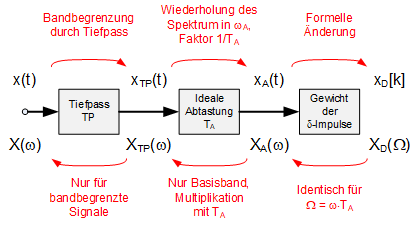
\includegraphics[width=0.5\textwidth]{Kapitel7/Bilder/image14.png}}
  \caption{Zusammenhang zwischen den Spektren des zeitkontinuierlichen Signals x(t), des abgetasteten Signals x${}_{A}$(t) und der Fourier-Transformierten der entsprechenden Folge x${}_{D}$[k]}
  \label{fig:SignalflussFT}
\end{figure}

\noindent Das zeitkontinuierliche Signal x(t) besitzt ein Spektrum X($\omega$). Um das Abtasttheorem zu erf\"{u}llen, wird es mit einem Tiefpass bandbegrenzt. Es entsteht das Signal x${}_{TP}$(t) mit dem Spektrum X${}_{TP}$($\omega$). Wegen der Abtastung ist das Spektrum X${}_{A}$($\omega$) periodisch in $\omega_{A}$ und mit dem Kehrwert der Abtastzeit 1/T${}_{A}$ skaliert. Die Folge x${}_{D}$[k] der Abtastwerte besitzt das Spektrum X${}_{D}$($\Omega$), das f\"{u}r $\Omega$ = $\omega\cdot$T${}_{A}$ dem Spektrum X${}_{A}$($\omega$) entspricht. Das Basisband von dem Spektrum X${}_{A}$($\omega$) entspricht dem Spektrum X${}_{TP}$($\omega$) und, wenn das Signal x(t) bandbegrenzt ist, auch dem Spektrum X($\omega$). Dieser Zusammenhang der verschiedenen Signale und ihrer Spektren wird an einem Beispiel illustriert.\bigskip

\noindent
\colorbox{lightgray}{%
\arrayrulecolor{white}%
\renewcommand\arraystretch{0.6}%
\begin{tabular}{ wl{16.5cm} }
{\fontfamily{phv}\selectfont{Beispiel: Zusammenhang zwischen Spektren zeitkontinuierlicher Signale und Signalfolgen}}
\end{tabular}%
}\medskip

\noindent Gegeben ist ein kausales, zeitkontinuierliches Signal

\begin{equation}\label{eq:sevenninetyteight}
x\left(t\right)=\left(e^{-t} -e^{-2\cdot t} \right)\cdot \sigma \left(t\right)
\end{equation}

\noindent Das Signal besitzt die Laplace-Transformierte 

\begin{equation}\label{eq:sevenninetytnine}
X\left(s\right)=\frac{1}{s+1} -\frac{1}{s+2} =\frac{1}{s+1} \cdot \frac{1}{s+2}
\end{equation}

\noindent Da die Laplace-Transformierte nur Pole in der negativen Halbebene besitzt, ergibt sich das Spektrum X($\omega$) zu

\begin{equation}\label{eq:sevenonehundred}
X\left(\omega \right)=\frac{1}{j\cdot \omega +1} \cdot \frac{1}{j\cdot \omega +2} =\frac{1}{2-\omega ^{2} +3\cdot j\cdot \omega}
\end{equation}

\noindent Das zeitkontinuierliche Signal x(t) sowie der Betrag des zugeh\"{o}rigen Spektrums {\textbar}X($\omega$){\textbar} sind in Bild \ref{fig:VergleichSpektrumSignaleFolgen1} dargestellt.

\begin{figure}[H]
  \centerline{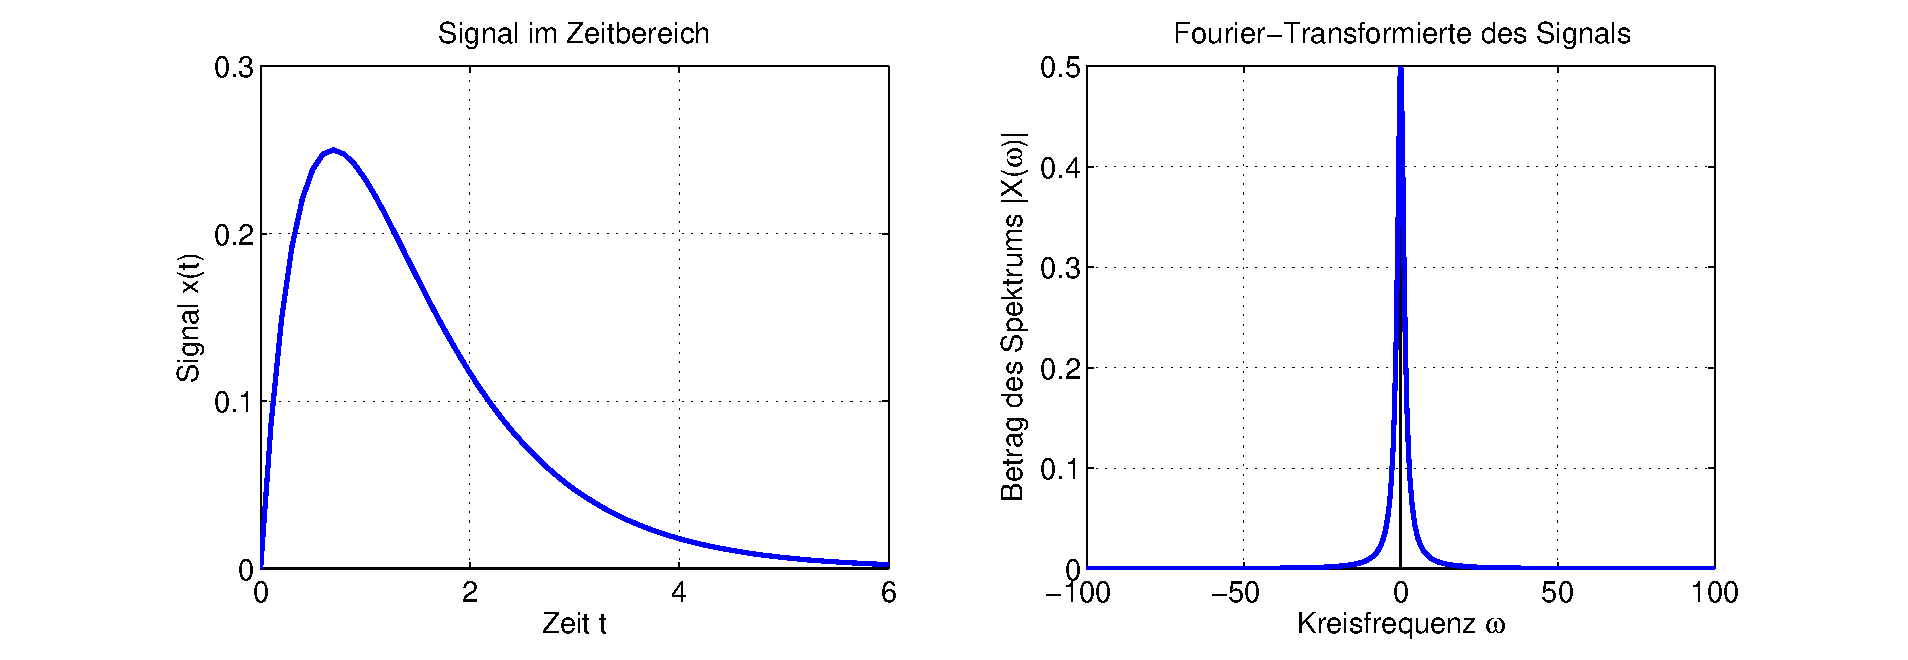
\includegraphics[width=1\textwidth]{Kapitel7/Bilder/image15.eps}}
  \caption{Zeitkontinuierliches Signal x(t) sowie der Betrag des zugeh\"{o}rigen Spektrums {\textbar}X($\omega$){\textbar}}
  \label{fig:VergleichSpektrumSignaleFolgen1}
\end{figure}

\noindent Das Signal wird mit einer Abtastzeit T${}_{A}$ = $\pi$/25 abgetastet. Dadurch wird das Spektrum periodisch in $\omega_{A}$ = 50 wiederholt und mit dem Faktor 1/T${}_{A}$ = 25/$\pi$ multipliziert. Das Spektrum des ideal abgetasteten Signals x${}_{A}$(t) ist in Bild \ref{fig:VergleichSpektrumSignaleFolgen2} dargestellt.

\begin{figure}[H]
  \centerline{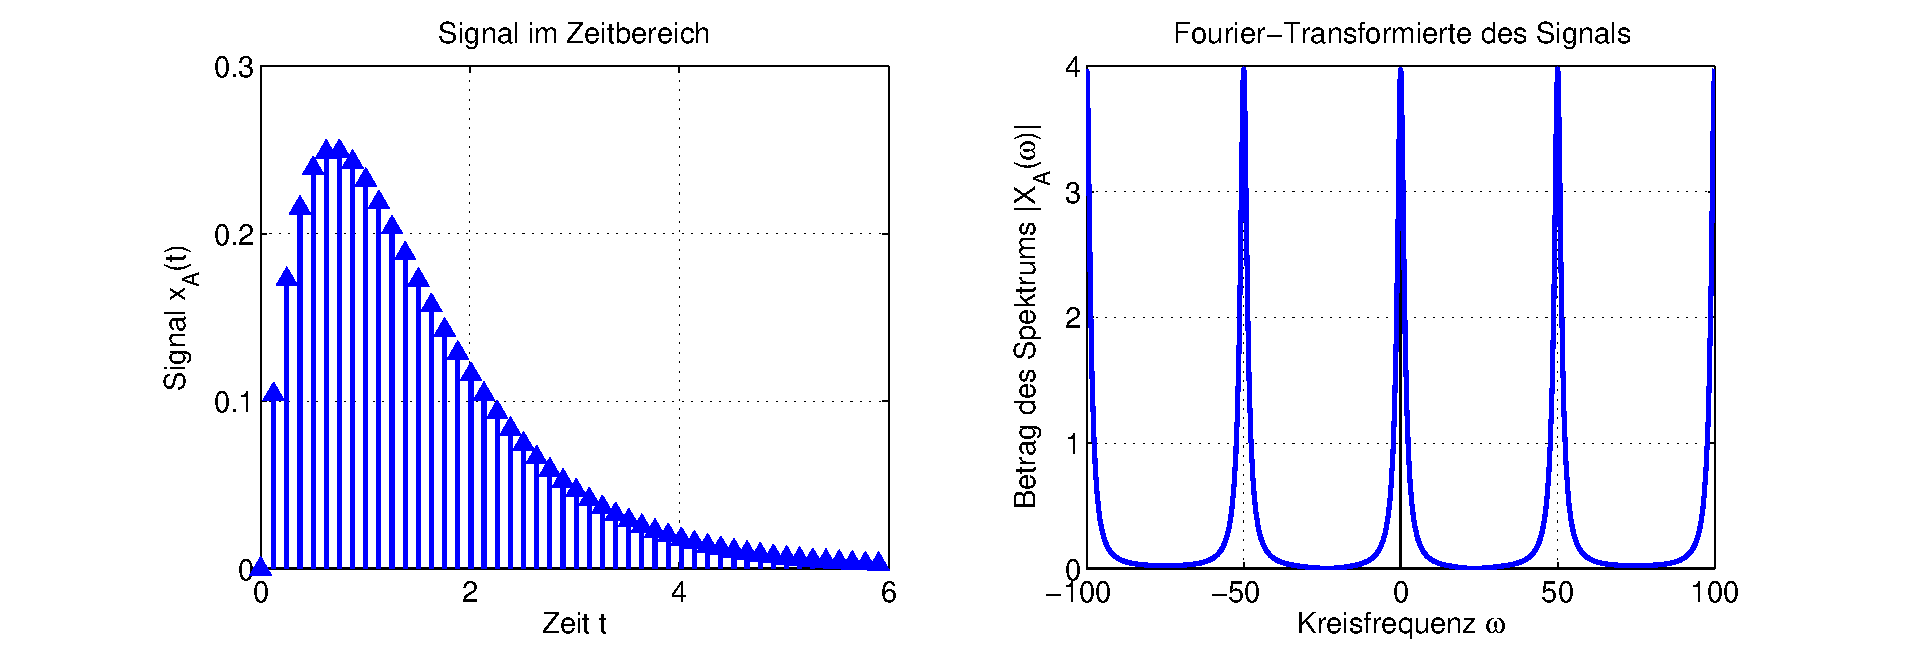
\includegraphics[width=1\textwidth]{Kapitel7/Bilder/image16.eps}}
  \caption{Ideal abgetastetes Signal x${}_{A}$(t) sowie der Betrag des zugeh\"{o}rigen Spektrums {\textbar}X${}_{A}$($\omega$){\textbar}}
  \label{fig:VergleichSpektrumSignaleFolgen2}
\end{figure}

\noindent Das Spektrum der zugeh\"{o}rigen Signalfolge 

\begin{equation}\label{eq:sevenonehundredone}
x_{D} \left[k\right]=\left(e^{-k\cdot T_{A} } -e^{-2\cdot k\cdot T_{A} } \right)\cdot \sigma \left[k\right]
\end{equation}

\noindent ist kontinuierlich und errechnet sich \"{u}ber die Definitionsgleichung der Fourier-Transformation f\"{u}r Folgen zu

\begin{equation}\label{eq:sevenonehundredtwo}
X_{D} \left(\Omega \right)=\sum _{k=-\infty }^{\infty }x_{D} \left[k\right]\cdot e^{-j\cdot \Omega \cdot k}  =\sum _{k=-\infty }^{\infty }\left(e^{-k\cdot T_{A} } -e^{-2\cdot k\cdot T_{A} } \right)\cdot \sigma \left[k\right]\cdot e^{-j\cdot \Omega \cdot k}
\end{equation}

\noindent Da es sich um eine kausale Folge handelt, kann die Summe auf zwei geometrische Reihen zur\"{u}ckgef\"{u}hrt und berechnet werden.

\begin{equation}\label{eq:sevenonehundredthree}
\begin{split}
X_{D} \left(\Omega \right) &=\sum _{k=0}^{\infty }\left(e^{-k\cdot T_{A} } -e^{-2\cdot k\cdot T_{A} } \right)\cdot e^{-j\cdot \Omega \cdot k}  =\sum _{k=0}^{\infty }e^{-k\cdot T_{A} } \cdot e^{-j\cdot \Omega \cdot k}  -\sum _{k=0}^{\infty }e^{-2\cdot k\cdot T_{A} } \cdot e^{-j\cdot \Omega \cdot k} \\
&=\sum _{k=0}^{\infty }\left(e^{-T_{A}-j\Omega} \right)^{k}-\sum _{k=0}^{\infty }\left(e^{-2\cdot T_{A}-j\Omega} \right)^{k}=\frac{1}{1-e^{-T_{A}-j\Omega}}-\frac{1}{1-e^{-T_{A}-j\Omega}}
\end{split}
\end{equation}

\noindent Bild \ref{fig:VergleichSpektrumSignaleFolgen3} zeigt die Signalfolge x${}_{D}$[k] und den Betrag des Spektrums der Signalfolge {\textbar}X${}_{D}$($\Omega$){\textbar} im Vergleich zum Spektrum X${}_{A}$($\omega$) des ideal abgetasteten Signals x${}_{A}$(t), wobei X${}_{A}$($\omega$) mit normierter Frequenz dargestellt ist.

\begin{figure}[H]
  \centerline{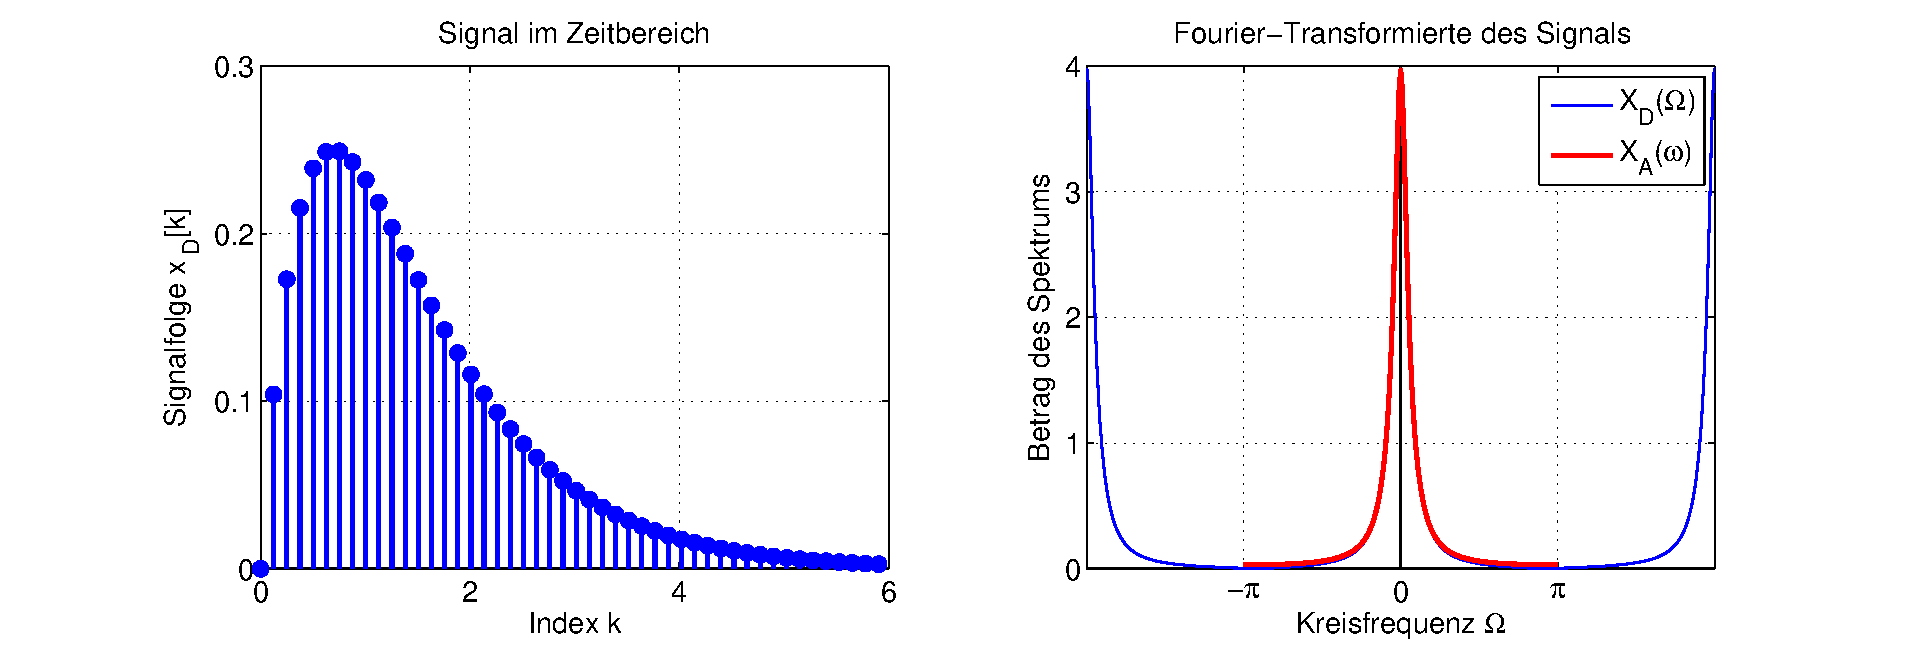
\includegraphics[width=1\textwidth]{Kapitel7/Bilder/image17.eps}}
  \caption{Folge der Abtastwert x${}_{D}$[k] sowie der Betrag des zugeh\"{o}rigen Spektrums {\textbar}X${}_{D}$($\Omega$){\textbar}}
  \label{fig:VergleichSpektrumSignaleFolgen3}
\end{figure}

\noindent Ein Vergleich der unterschiedlichen Spektren zeigt, dass mit der Fourier-Transformation der Signalfolge x${}_{D}$[k] das Spektrum des zeitkontinuierlichen Signals berechnet werden kann, wenn das Abtasttheorem eingehalten wird. Allerdings m\"{u}ssen dazu unendlich viele Abtastwerte x${}_{D}$[k] vorliegen, was normalerweise nicht der Fall ist. Die Bestimmung des Spektrums eines Signals bei einer endlichen Anzahl von Abtastwerten wird in Kapitel 1 diskutiert.

\subsubsection{Zusammenhang zwischen z-Transformation und Fourier-Transformation kausaler Signalfolgen}

\noindent Bei dem Vergleich der Definitionsgleichungen der z-Transformation 

\begin{equation}\label{eq:sevenonehundredfour}
X\left(z\right)=\sum _{k=0}^{\infty }x\left[k\right]\cdot z^{-k}
\end{equation}

\noindent und der Fourier-Transformation von kausalen Folgen 

\begin{equation}\label{eq:sevenonehundredfive}
X\left(\Omega \right)=\sum _{k=0}^{\infty }x\left[k\right]\cdot e^{-j\cdot k\cdot \Omega }
\end{equation}

\noindent f\"{a}llt auf, dass die Variable z der z-Transformation bei der Fourier-Transformation von kausalen Folgen durch den Ausdruck e${}^{j}$ ersetzt wird. Grafisch gesehen wird bei dem \"{U}bergang von der z-Transformierten auf die Fourier-Transformierte das Spektrum \"{u}ber dem Einheitskreis abgewickelt. 

\clearpage

\noindent
\colorbox{lightgray}{%
\arrayrulecolor{white}%
\renewcommand\arraystretch{0.6}%
\begin{tabular}{ wl{16.5cm} }
{\fontfamily{phv}\selectfont{Beispiel: Zusammenhang zwischen z-Transformation und Fourier-Transformation von Signalfolgen}}
\end{tabular}%
}\medskip

\noindent Dieser Sachverhalt wird anhand eines Signals mit der z-Transformierten 

\begin{equation}\label{eq:sevenonehundredsix}
X\left(z\right)=\frac{z^{2} }{z^{2} -z+0.5}
\end{equation}

\noindent anschaulich dargestellt. Bild \ref{fig:VergleichTransformationzFourier1} zeigt die Pol-Nullstellenverteilung der z-Transformierten X(z).

\begin{figure}[H]
  \centerline{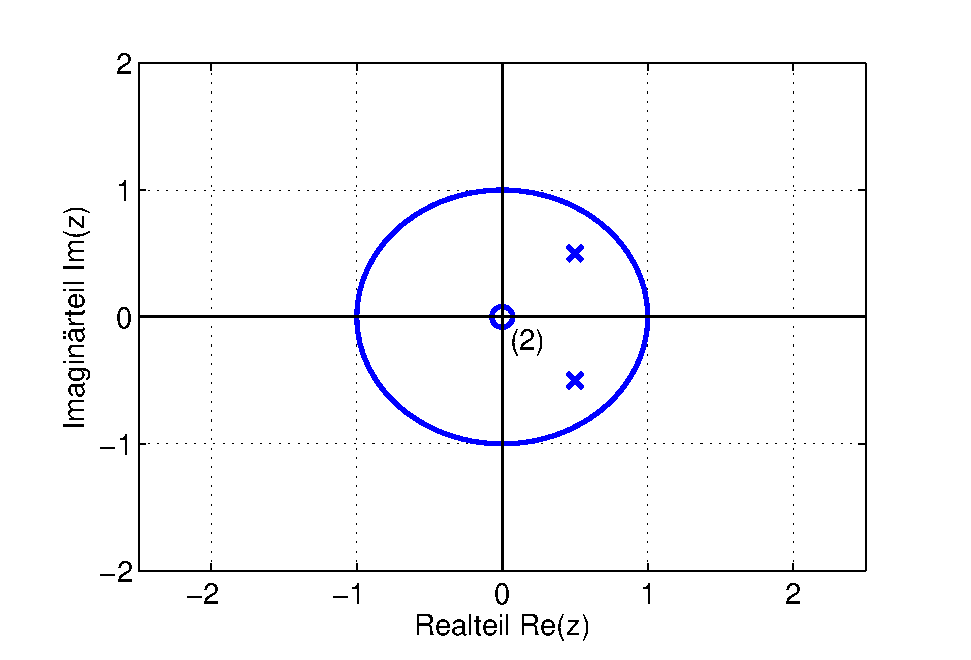
\includegraphics[width=0.5\textwidth]{Kapitel7/Bilder/image18.eps}}
  \caption{Pol-Nullstellenverteilung der z-Transformierten X(z)}
  \label{fig:VergleichTransformationzFourier1}
\end{figure}

\noindent Die z-Transformierte X(z) hat ein konjugiertes Polpaar an der Stelle $\alpha$ = 0.5 $\mathrm{\pm}$ 0.5$\cdot$j und eine doppelte Nullstelle $\beta$ = 0. Beide Pole liegen innerhalb des  Einheitskreises. Der Betrag der z-Transformierten und der Betrag der Fourier-Transformierten werden in Bild \ref{fig:VergleichTransformationzFourier2} verglichen.

\begin{figure}[H]
  \centerline{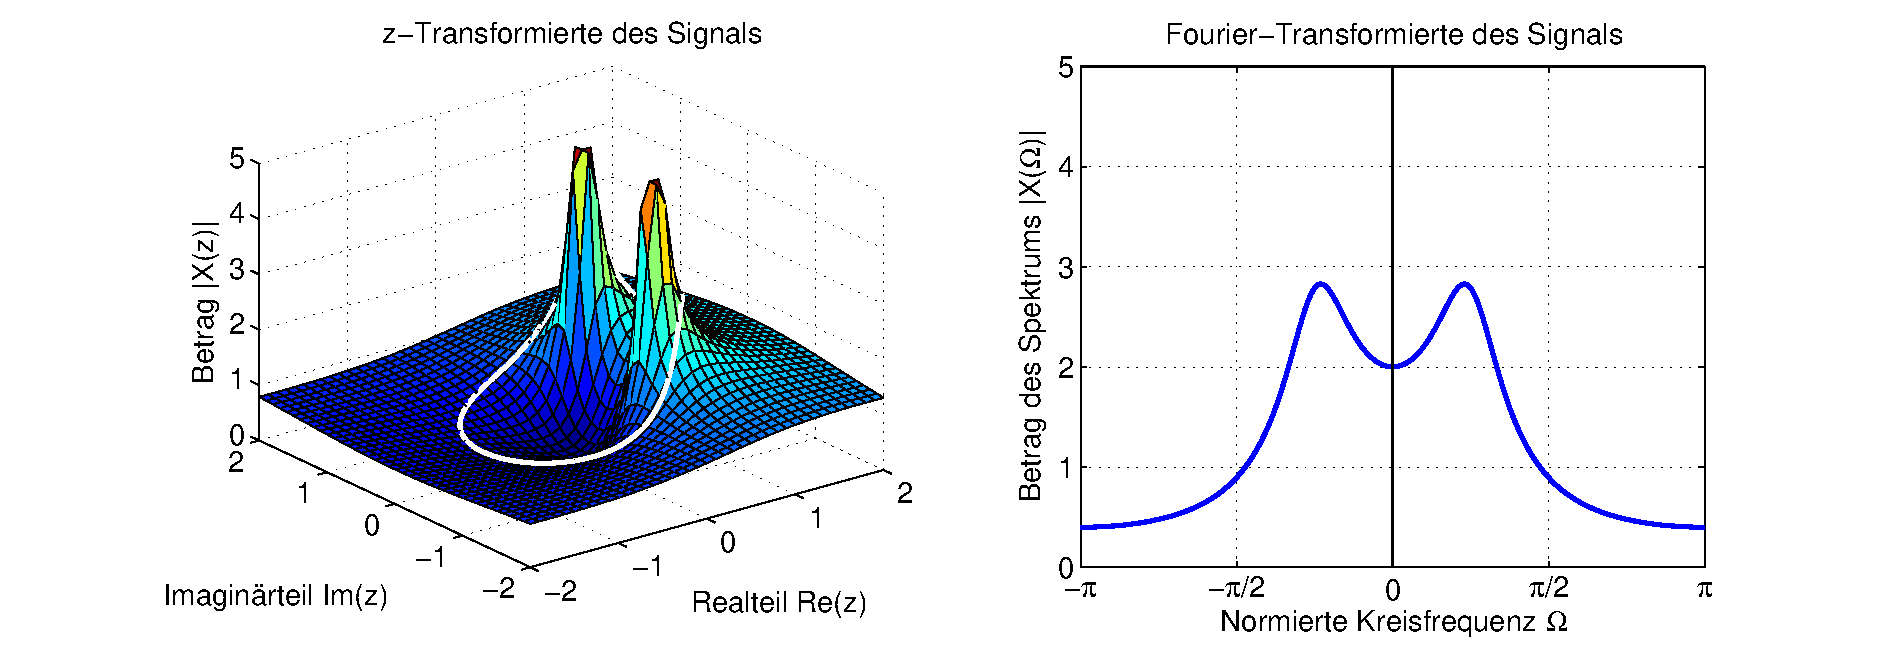
\includegraphics[width=1\textwidth]{Kapitel7/Bilder/image19.eps}}
  \caption{Vergleich des Betrags der z-Transformierten X(z) und der Fourier-Transformierten}
  \label{fig:VergleichTransformationzFourier2}
\end{figure}

\noindent In der linken Grafik ist der Betrag der z-Transformierten dargestellt. An den beiden Polen wird der Betrag der \"{U}bertragungsfunktion unendlich gro{\ss}, in der Grafik wird er auf den Wert 5 begrenzt. Au{\ss}erdem ist mit dem wei{\ss}en Kreis der Betrag der \"{U}bertragungsfunktion \"{u}ber dem Einheitskreis dargestellt. Die Abwicklung dieses Kreises entspricht dem in der rechten Grafik dargestellten Betrag des Spektrums. Der Betrag des Spektrums ist nahe den Polen gro{\ss} und sinkt mit steigendem Abstand zu den Polen ab.

\clearpage

\noindent Bild \ref{fig:VergleichTransformationzFourier3} stellt die Phase der z-Transformierten und die Phase der Fourier-Transformierten dar.

\begin{figure}[H]
  \centerline{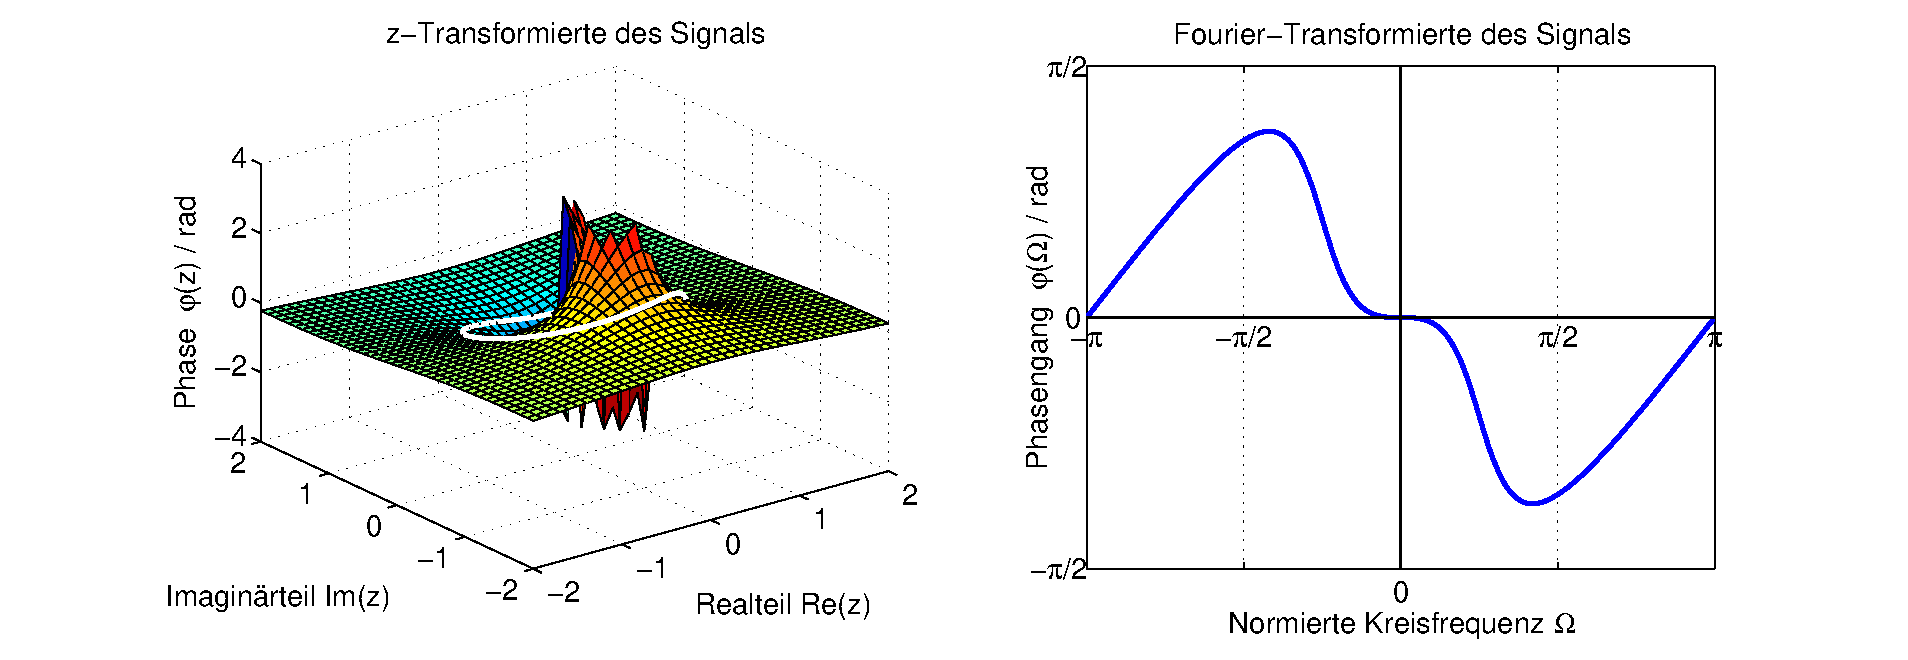
\includegraphics[width=1\textwidth]{Kapitel7/Bilder/image20.eps}}
  \caption{Vergleich der Phase der z-Transformierten X(z) und der Fourier-Transformierten}
  \label{fig:VergleichTransformationzFourier3}
\end{figure}

\noindent In der linken Grafik ist die Phase der z-Transformierten dargestellt. Zwischen der Nullstelle und den Polen im Koordinatenursprung \"{a}ndert sich die Phase von - $\pi$ auf $\pi$. Aufgrund der r\"{a}umlichen Darstellung ist dieser Sprung leider verdeckt. Mit dem wei{\ss}en Kreis ist die Phase der \"{U}bertragungsfunktion \"{u}ber dem Einheitskreis dargestellt. Die Abwicklung dieses Kreises entspricht der in der rechten Grafik dargestellten Phase des Spektrums. Die Phasen\"{a}nderung des Spektrums ist nahe den Polen gro{\ss} und sinkt mit steigendem Abstand zu den Polen ab.\newline

\noindent Der Vergleich zeigt, dass die Fourier-Transformierte einer Folge aus der z-Transformierten \"{u}ber die Substitution z = e${}^{j}$ gewonnen werden kann. Dazu ist es allerdings erforderlich, dass der Einheitskreis im Konvergenzbereich der z-Transformierten liegt. Nach den Ausf\"{u}hrungen zur z-Transformation in Kapitel 5.1 ist das der Fall, wenn alle Pole der z-Transformierten im Einheitskreis liegen.\bigskip

\noindent
\colorbox{lightgray}{%
\arrayrulecolor{white}%
\renewcommand\arraystretch{0.6}%
\begin{tabular}{ wl{16.5cm} }
{\fontfamily{phv}\selectfont{Beispiel: Berechnung der Fourier-Transformierten aus der z-Transformierten}}
\end{tabular}%
}\medskip

\noindent Die Fourier-Transformierte eines Signals mit der z-Transformierten 

\begin{equation}\label{eq:sevenonehundredseven}
X\left(z\right)=\frac{z^{2} }{z^{2} -z+0.5}
\end{equation}

\noindent soll berechnet werden. Die Pole der z-Transformierten liegen nach Bild 7.18 innerhalb des Einheitskreises. Damit ergibt sich die Fourier-Transformierte aus

\begin{equation}\label{eq:sevenonehundredeight}
X\left(\Omega \right)=\left. X\left(z\right)\right|_{z=e^{j\cdot \Omega } } =\frac{e^{j\cdot 2\cdot \Omega } }{e^{j\cdot 2\cdot \Omega } -e^{j\cdot \Omega } +0.5}
\end{equation}

\noindent Der Betrag des Spektrums ist bereits in Bild\ref{fig:VergleichTransformationzFourier2} dargestellt.
\clearpage
\subsection{Berechnung von Korrespondenzen der Fourier-Transformation von Signalfolgen}

\noindent In den vorangegangenen Abschnitten werden unterschiedliche Methoden zur Berechnung von Korrespondenzen der Fourier-Transformation von Signalfolgen diskutiert. Zur besseren \"{U}bersicht stellt Bild \ref{fig:MethodenFourierTransformation} die unterschiedlichen Methoden zusammen und gibt die Bedingungen an, unter denen die entsprechenden Methoden angewendet werden k\"{o}nnen.

\begin{figure}[H]
  \centerline{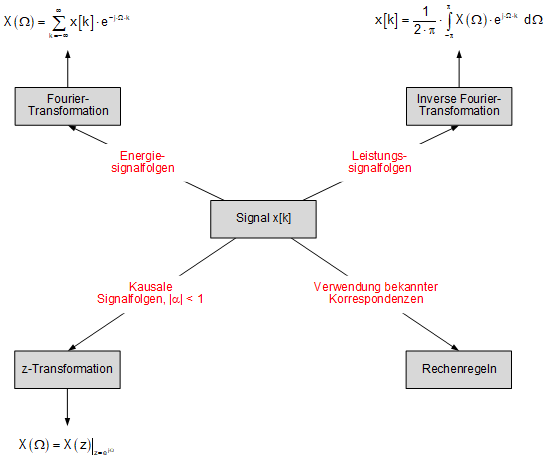
\includegraphics[width=0.8\textwidth]{Kapitel7/Bilder/image21.png}}
  \caption{Methoden zur Berechnung von Korrespondenzen der Fourier-Transformation von Signalfolgen}
  \label{fig:MethodenFourierTransformation}
\end{figure}

\noindent Korrespondenzen der Fourier-Transformation k\"{o}nnen \"{u}ber die Definitionsgleichungen der Fourier-Transformation und der inversen Fourier-Transformation berechnet werden, wenn die entsprechenden Integrale konvergieren. Bei Energiesignalfolgen ist das f\"{u}r die Definitionsgleichung der Fourier-Transformation generell der Fall. Bei Leistungssignalfolgen wird ausgehend von einer Fourier-Transformierten X($\Omega$) die zugeh\"{o}rige Signalfolge x[k] bestimmt.

\noindent Aus der z-Transformierten X(z) ergibt sich die Fourier-Transformierte X($\Omega$) durch Substitution, wenn die Signalfolge x[k] kausal ist und die Pole von X(z) im Einheitskreis ({\textbar}$\alpha${\textbar} $\mathrm{<}$ 1).

\clearpage

\subsection{Literatur}


\subsubsection{Literaturstellen mit besonders anschaulicher Darstellung}

\begin{tabular}{|p{0.6in}|p{5.7in}|} \hline 
[Lyon04] & Lyons, Richard G.: Understanding Digital Signal Processing,\newline Prentice Hall, New Jersey, 2004 \\ \hline 
[Schei05] & Scheithauer, Rainer: Signale und Systeme,\newline 2. Auflage, B.G. Teubner Stuttgart, 2005 \\ \hline 
[Stea99] & Stearns, Samuel: Digitale Verarbeitung analoger Signale,\newline 7. Auflage, Oldenbourg Verlag M\"{u}nchen, 1999 \\ \hline 
\end{tabular}

\subsubsection{Literaturstellen mit praktischen Anwendungen}

\begin{tabular}{|p{0.6in}|p{5.7in}|} \hline 
[Wern08] & Werner, Martin: Signale und Systeme,\newline Vieweg Studium Technik, Wiesbaden, 2008 \\ \hline 
[Meye08] & Meyer, Martin: Signalverarbeitung -- Analoge und digitale Signal, Systeme und Filter,\newline Vieweg Studium Technik, Wiesbaden, 2008 \\ \hline 
\end{tabular}

\subsubsection{Literatur zu MATLAB}

\begin{tabular}{|p{0.6in}|p{5.7in}|} \hline 
[Schw07] & Schweizer, Wolfgang: MATLAB kompakt,\newline Oldenbourg Verlag M\"{u}nchen, 2007 \\ \hline 
[Stei07] & Stein, Ulrich: Einstieg in das Programmieren mit MATLAB,\newline Fachbuchverlag Leipzig, 2007 \\ \hline 
\end{tabular}

\subsubsection{Weiterf\"{u}hrende Literatur}

\begin{tabular}{|p{0.6in}|p{5.7in}|} \hline 
[Oppe04] & Oppenheim, Alan: Zeitdiskrete Signalverarbeitung,\newline 2. \"{u}berarbeitete Auflage, Pearson Studium, 2004 \\ \hline 
[Kamm98] & Kammeyer, Karl: Digitale Signalverarbeitung,\newline B.G. Teubner Stuttgart, 1998 \\ \hline 
\end{tabular}